%% ----------------------------------------------------------------
%% Thesis.tex -- MAIN FILE (the one that you compile with LaTeX) MAIN REPORT
%% ---------------------------------------------------------------- 

% Set up the document
\documentclass[a4paper, 12pt, twoside]{Thesis}  % Use the "Thesis" style, based on the ECS Thesis style by Steve Gunn
\graphicspath{Figures/}  % Location of the graphics files (set up for graphics to be in PDF format)
%\usepackage{url}
%\PassOptionsToPackage{hyphens}{url}
\usepackage{hyperref} 
% Include any extra LaTeX packages required
\usepackage[square, numbers, comma, sort&compress]{natbib}  % Use the "Natbib" style for the references in the Bibliography\cite{Reference2}
\usepackage{verbatim}  % Needed for the "comment" environment to make LaTeX comments
\usepackage{vector}  % Allows "\bvec{}" and "\buvec{}" for "blackboard" style bold vectors in maths

\hypersetup{urlcolor=black, colorlinks=true}  % Colours hyperlinks in blue, but this can be distracting if there are many links.

\usepackage{float}
\usepackage{listings}
\usepackage{lscape}
\usepackage{multirow}
%\usepackage{lineno}
%\linenumbers
%% ----------------------------------------------------------------
\begin{document}
\frontmatter      % Begin Roman style (i, ii, iii, iv...) page numbering

% Set up the Title Page
\title  {Towards Presence in Telerobotics: Real-time Image Abstraction for Virtual Reality}

\authors  {\texorpdfstring
            {Adam Melvin}
            {Author Name}
            }
\addresses  {\groupname\\\deptname\\\univname}  % Do not change this here, instead these must be set in the "Thesis.cls" file, please look through it instead
\date       {\today}
\subject    {}
\keywords   {}

\maketitle
%% ----------------------------------------------------------------

\setstretch{1.3}  % It is better to have smaller font and larger line spacing than the other way round

% Define the page headers using the FancyHdr package and set up for one-sided printing
\fancyhead{}  % Clears all page headers and footers
\rhead{\thepage}  % Sets the right side header to show the page number
\lhead{}  % Clears the left side page header

\pagestyle{fancy}  % Finally, use the "fancy" page style to implement the FancyHdr headers


%% ----------------------------------------------------------------

% The Abstract Page
%\addtotoc{Abstract}  % Add the "Abstract" page entry to the Contents
\abstract{
%\addtocontents{toc}{\vspace{1em}}  % Add a gap in the Contents, for aesthetics

The application of Virtual Reality (VR) to telerobotics is a current area of study due to a desire for the increased spacial awareness VR provides. However, attempts to implement such a system using standard teleoperation techniques result in sub-par performance and an uncomfortable experience for the user; the benefits of a VR based system are entirely eliminated. The system proposed by this project incorporates elements of data abstraction to produce abstractions of the environment. This process reduces the performance requirements of providing the user presence within the telerobot's space such that reasonable spacial awareness can be achieved.

\clearpage  % Abstract ended, start a new page
%% ----------------------------------------------------------------

\pagestyle{fancy}  %The page style headers have been "empty" all this time, now use the "fancy" headers as defined before to bring them back


%% ----------------------------------------------------------------
\lhead{\emph{Contents}}  % Set the left side page header to "Contents"
\tableofcontents  % Write out the Table of Contents

%% ----------------------------------------------------------------
\lhead{\emph{List of Figures}}  % Set the left side page header to "List if Figures"
\listoffigures  % Write out the List of Figures

%% ----------------------------------------------------------------

% The Acknowledgements page, for thanking everyone
\acknowledgements{
%\addtocontents{toc}{\vspace{1em}}  % Add a gap in the Contents, for aesthetics

I would like to thank Klaus-Peter Zauner for his incredible help and support. I would also like to thank Tom Darlison and Lawrence Gray for their help and for being expert "rubber ducks". Finally, I would like to thank the users of the Building 16 labs for treating my rover driving around with the utmost patience.

}
\clearpage  % End of the Acknowledgements
%% ----------------------------------------------------------------

%% ----------------------------------------------------------------
\mainmatter	  % Begin normal, numeric (1,2,3...) page numbering
\pagestyle{fancy}  % Return the page headers back to the "fancy" style

% Include the chapters of the thesis, as separate files
% Just uncomment the lines as you write the chapters

\chapter{Introduction}
\lhead{\emph{Introduction}}

The desire for a feeling of presence \cite{presence} within a space that is not your own is one that drives much technological innovation. Whether it be within a virtual space such as in video games or immersion therapy, or within a different real world location as in telerobotics, greater presence allows the user to more naturally and intuitively interact with the presented environment as if they were truly there. In telerobotics in particular, where the aim can often be to interact with very dangerous or industrial environments, intuitive control is essential to safe and effective operation.

Virtual Reality (VR) is a technology spearheaded by the video games industry for use in immersive gaming application. Through the use of a tracked headset, giving the user the ability to freely look around a 3D space, it provide unparalleled presence within a virtual world- comparable to presence within a real, physical space \cite{loomis2016presence,McGlynn}. To be able to incorporate VR into teleoperation is therefore desirable, however, sending a video feed to the headset as if it were a normal monitor has been found to lead to motion sickness \cite{han2017design}. This is due to VR's high frame rate and low latency requirements. It's widely accepted that for a VR application to not cause motion sickness and headaches due to frame rate, it must maintain at least 90 frames per second (fps) \cite{FrameRate}; a minimum of 60 fps can also be acceptable \cite{Borg2013UsingAG}, but generally only for applications with little motion or when used by people with lower susceptibility to motion sickness. Unfortunately, to transmit 90 fps from a stereo camera rig (two images are required to perceive 3D) to the computer running the VR application has bandwidth requirements too high to be currently implementable outside the most expensive of designs.

The ability to look around the space independently is a major factor in providing presence to the user in VR. This can be achieved by mounting the stereo camera rig on a gimbal, however to build a gimbal that is able to track the angle of the user's head accurately and with low latency is, once again, expensive and challenging \cite{DORA}; if not implemented perfectly the user would experience significant sickness and dissociation from the space.

The aim of this project is to design and implement a VR based teleoperation system that utilises data abstraction to minimise the outlined technical issues, providing the foundations for future systems to be able to provide true presence to the user. To achieve this, each image is reduced down to its most essential features, reducing its size and therefore the required bandwidth significantly. Each image pair must then transmitted to a server and combined into a single 3D model of the space that could be looked around freely through the VR headset. As the camera feed is converted to a 3D model rather than displayed directly as images, the headset could run at the full 90fps even if the model is updating at a much slower rate.

The system (outlined in Figure \ref{fig:outline}) consists of 2 platforms- a server that runs a VR environment and reads user input, and a rover platform that is controlled from said environment and supplies the abstracted images the environment is built from. The rover (Figure \ref{fig:marvin}) is a simple drivable platform with a stereo camera gimbal mounted on it (adapted from one produced by previous students \cite{gimble}), and is the subject of Chapter \ref{chapter:rover}. The server is a powerful PC running Windows 10 \cite{windows} and a HTC Vive. The design of the program the server runs is the subject of Chapter \ref{chapter:server}. The data abstraction algorithm the system uses is novel, so its design and development is initially discussed in isolation in Chapter \ref{chapter:abstract} and then its application within the system addressed in Chapter \ref{chapter:rover}. The full system will be evaluated in Chapter \ref{chapter:eval}.

\begin{figure}[H]
    \begin{center}
      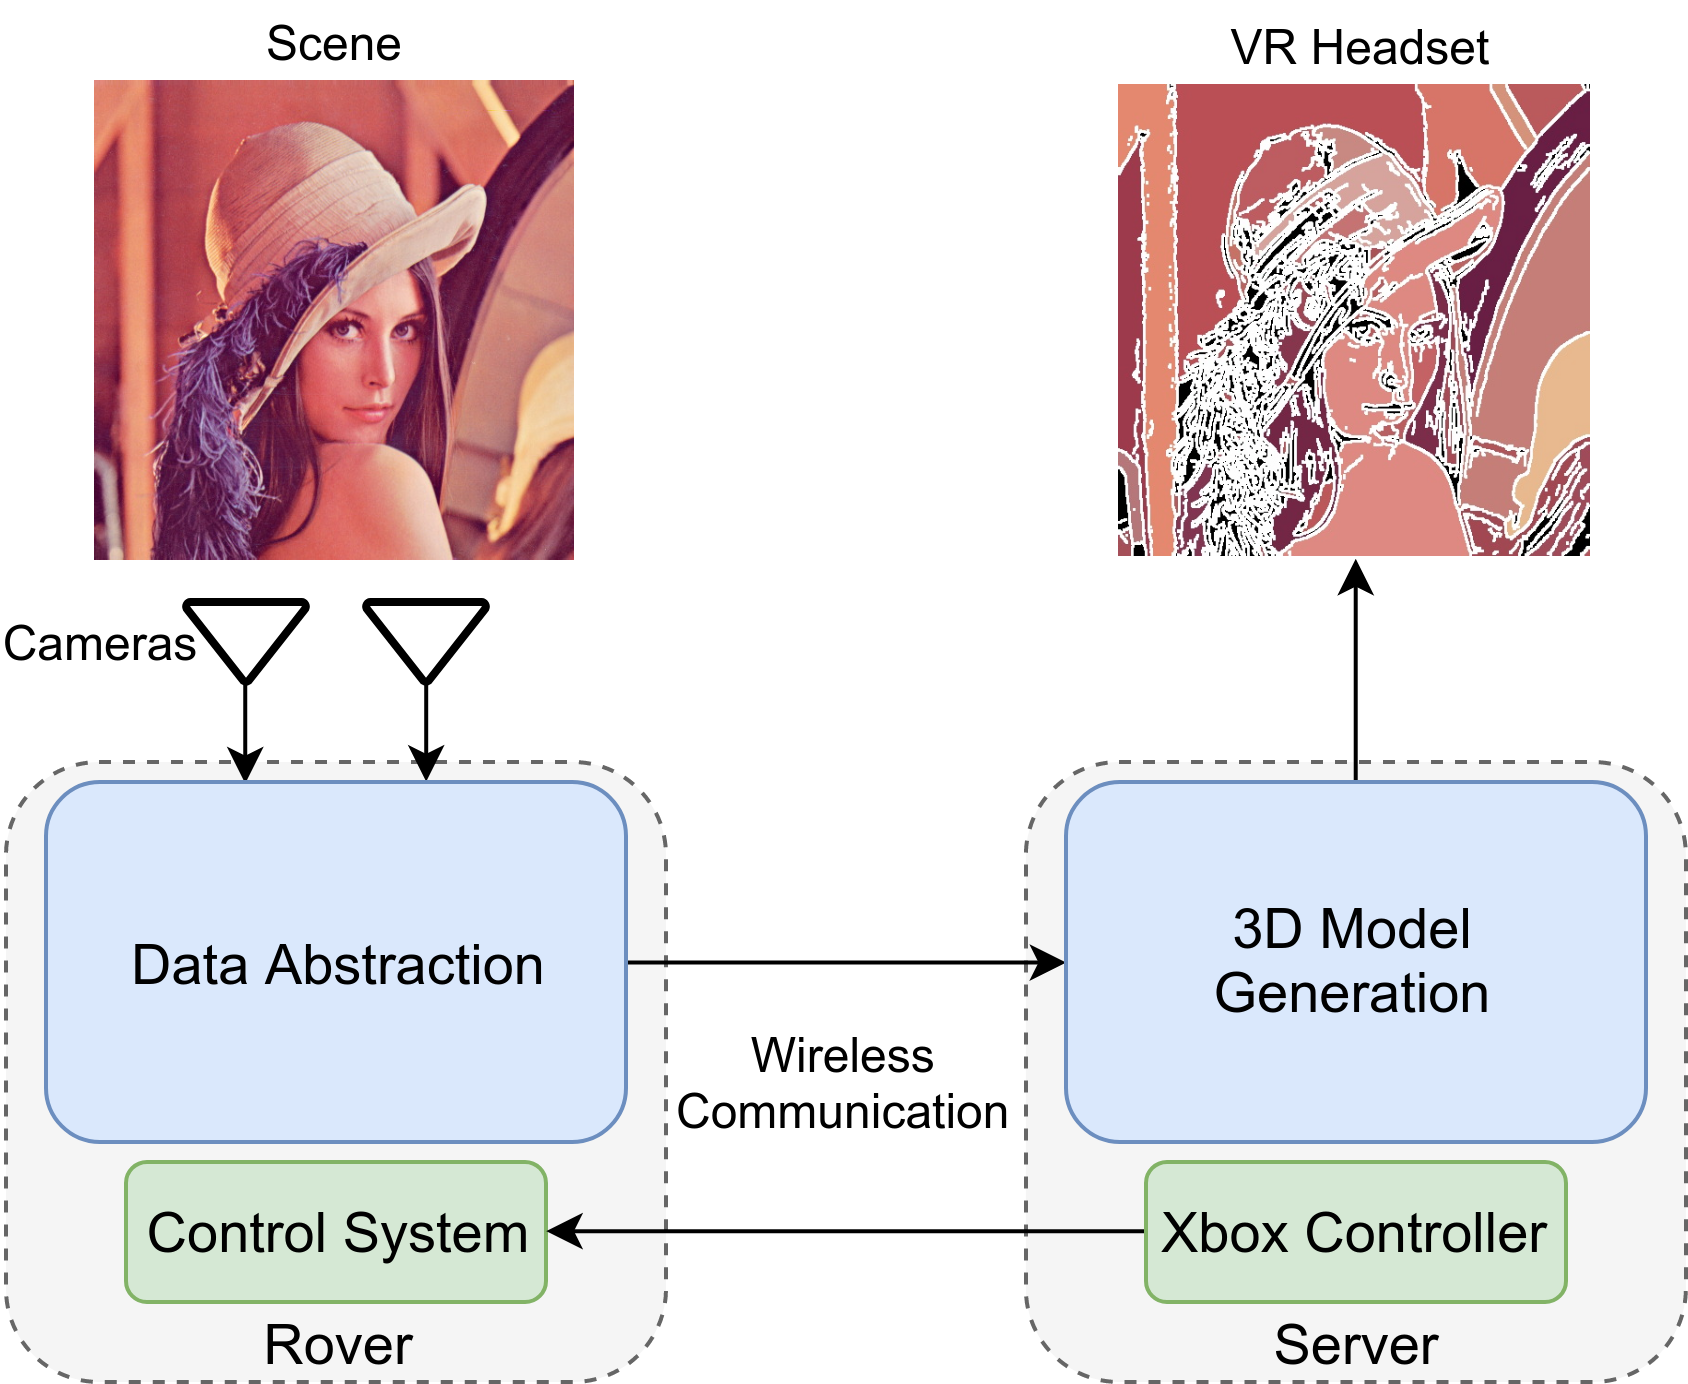
\includegraphics[width=0.9\textwidth]{Figures/Outline.png}
      \caption[System Outline]{System Outline.\textcolor{red}{[REPLACE PICS]}}
      \label{fig:outline}
    \end{center}
\end{figure}

\begin{figure}[H]
    \begin{center}
      \begin{tabular}{ c }
        \includegraphics[width=0.65\textwidth]{Figures/marvin.jpg} \\
        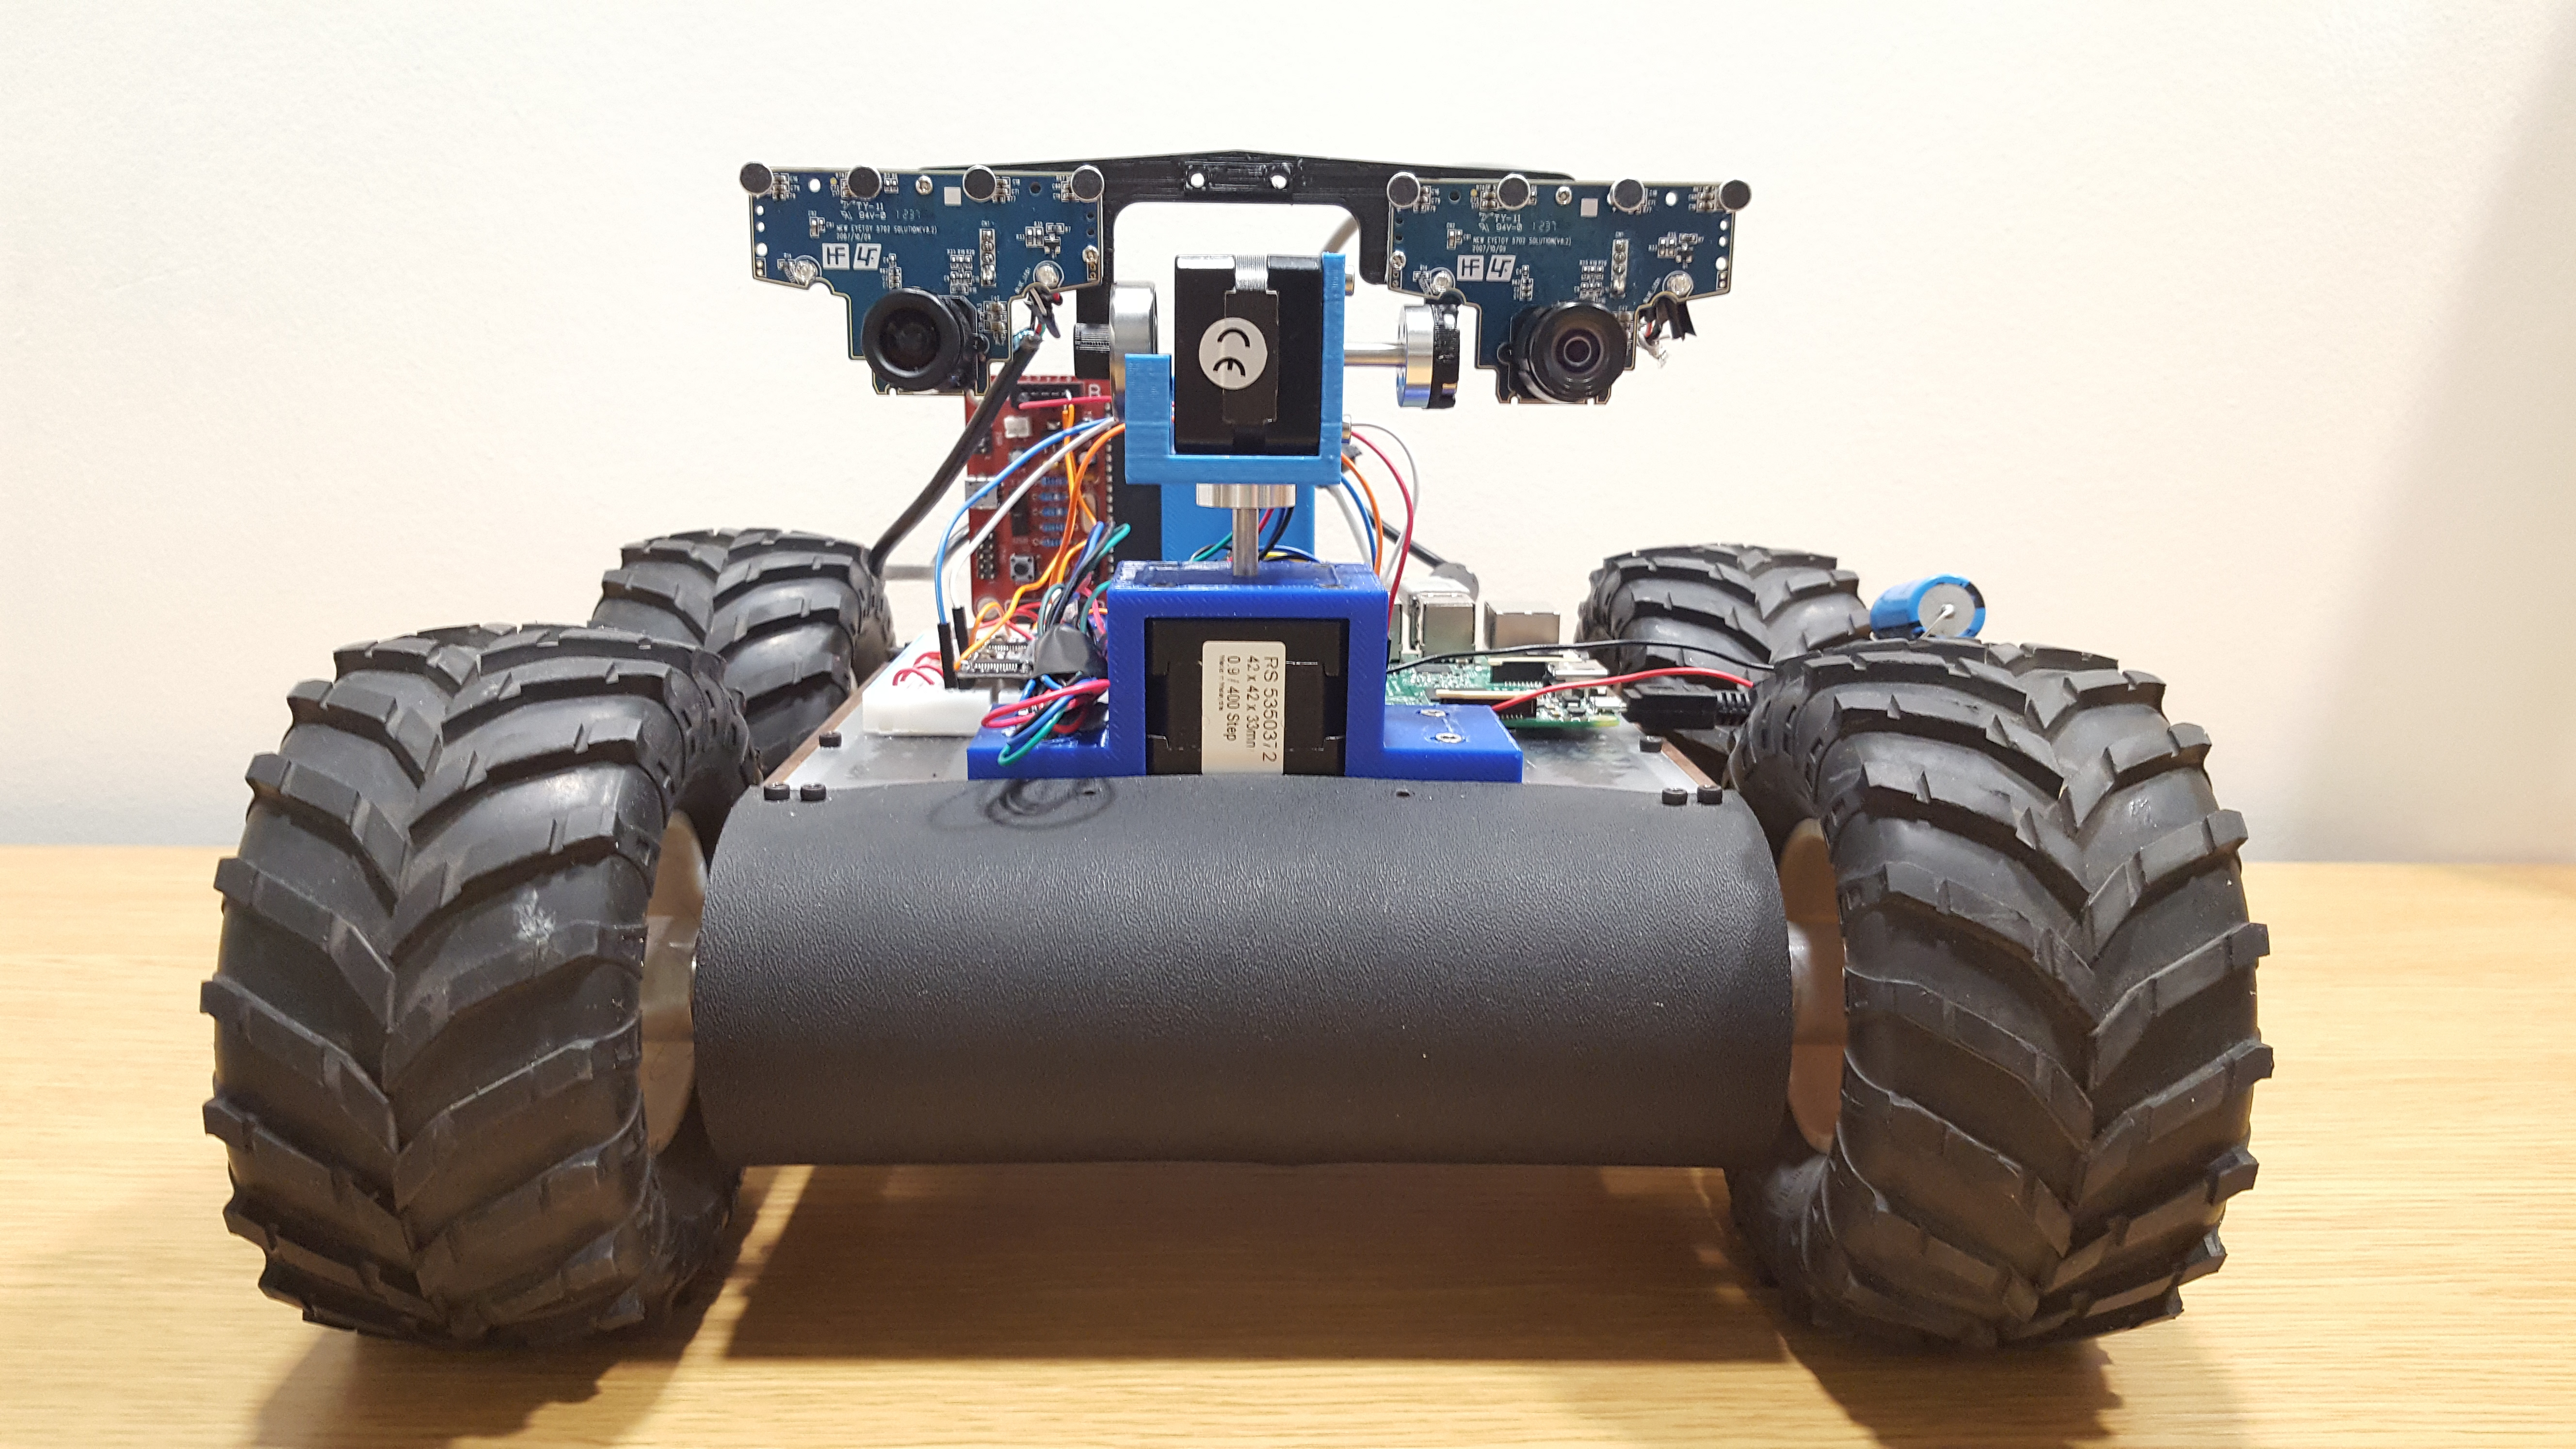
\includegraphics[width=0.65\textwidth]{Figures/marvinF.jpg} \\
        \includegraphics[width=0.65\textwidth]{Figures/marvinS.jpg} \\
        \includegraphics[width=0.65\textwidth]{Figures/marvinT.jpg}
      \end{tabular}
      \caption[Rover Pictures]{Rover Pictures.}
      \label{fig:marvin}
    \end{center}
\end{figure} % Introduction

\chapter{Background}
\lhead{\emph{Background}}

\section{Virtual Reality}

The term Virtual Reality (VR) refers to the generation of a 3D environment that can be interacted with by a user in a realistic fashion, with the aim of immersing the user in the environment as if it were the real world \cite{WhatVR}. While there are a large array of systems that can be considered VR, whenever the term is used in this report it is only referring to the head-mounted display (HMD) systems that have become popular in recent years with the release of the Oculus Rift \cite{Oculus} and the HTC Vive \cite{Vive} (Figure \ref{fig:Vive}). These are both consumer grade systems that are aimed at the immersive gaming market.

\begin{figure}[H]
    \begin{center}
    \begin{tabular}{ c c }
        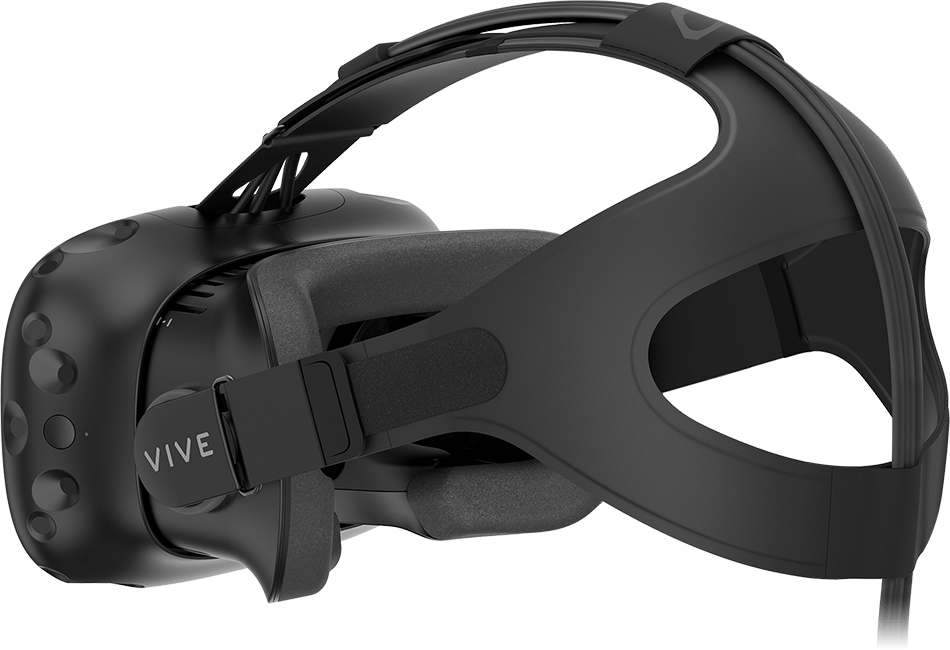
\includegraphics[width=0.4\textwidth]{Figures/vive.png} &
        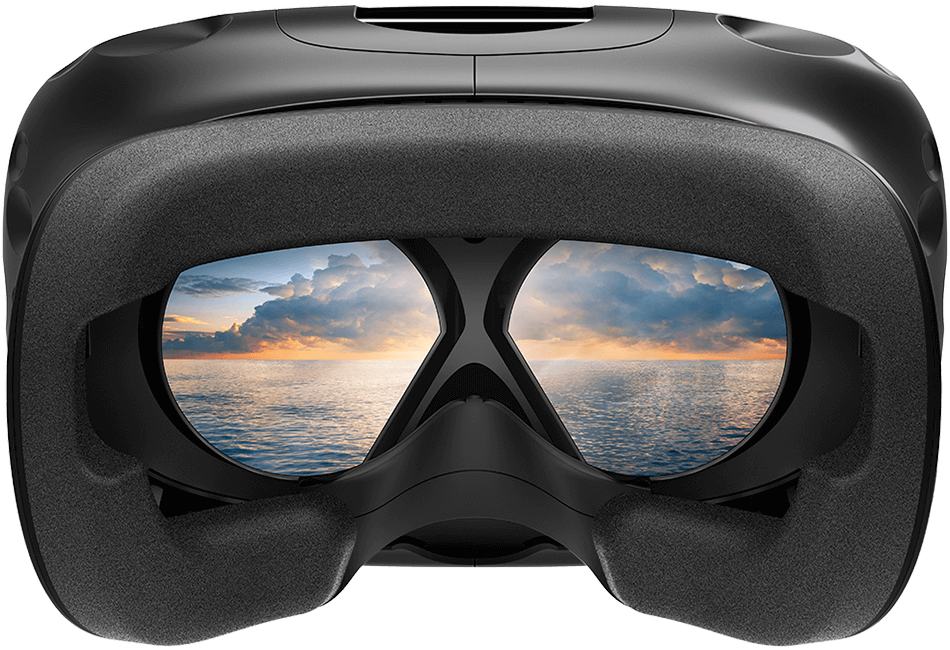
\includegraphics[width=0.4\textwidth]{Figures/vive2.png}
    \end{tabular}
    \caption[HTC Vive]{HTC Vive. Pictures of the Vive headset, reproduced from \cite{Vive}.}
    \label{fig:Vive}
    \end{center}
\end{figure}

HMD based systems display different images for each eye to provide the user with a sense of depth within the 3D environment, making the headset effectively operate like a pair of binoculars into the virtual world. The headset is also tracked in 3D space, and this movement translated into the 3D environment with low latency. These features, among others, are all implemented with the aim of providing the user with presence within the virtual space that is comparable to observing the real world.

Due to its availability at the University of Southampton and in my own home, the HTC Vive was used as the VR device in the development and implementation of the teleoperations system discussed in this report. 

\section{Telerobotics}

A telerobot is a robot controlled from a distance by a human operator \cite{sheridan1989telerobotics}. Telerobots are typically developed to undertake activities within environments that are too dangerous or costly for humans to work in. Typical fields of telerobotics research include deep-space exploration \cite{fong2017interactive}, deep-sea exploration \cite{huvenne2018rovs}, and handling radioactive materials \cite{smith2017radiation}.

\subsection{VR in Telerobotics}
\label{subsection:VRTele}

The use of HMDs in teleoperations is not a new concept; NASA's Robonaut 2 was sent to the International Space Station in 2011 and can be controlled through a headset that displays the output of the robot's head cameras \cite{Robonaut}, and flying drones by First Person View (FPV), an analogue video feed transmitted over radio to a HMD, has become popular in recent years \cite{FPV}. However, these systems are either incredibly expensive (Robonaut 2 is worth millions of dollars) or very limited (FPV systems are only capable of sending one low quality video stream over a short distance), and all suffer from the motion sickness issues discussed in Chapter \ref{chapter:intro}. While stereo camera FPV systems have been developed, so the user has depth perception and better presence in the drone's view, the motion sickness problem remains the major drawback of HMD based teleoperations systems \cite{2FPV}.

As previously established, motion sickness in VR is mitigated through high frame rates and low latency. However, VR based teleoperations systems are typically direct VR systems, so they display the video feeds provided by the telerobot's cameras directly in the headset. This entirely ties the frame rate and latency of the headset to the capabilities of the video transmission system, and only the most expensive and complicated systems will meet the strict requirements for comfortable VR and high spacial presence.

An alternate option to a direct system is an indirect system. This is one in which the video feed is abstracted from the headset in some way in the hope of providing improved comfort and awareness. Indirect systems can come in a variety of forms, such as placing the video feed on a virtual screen in the VR environment and controlling the robot using virtual controls laid out infront of the screen \cite{lipton2018baxter}, or a 3D map generated from a multi-line LiDAR and IMU \cite{wang2017novel} (Figure \ref{fig:VRTele}). These examples show the potential of indirect systems as a solution to VR based teleoperations, however neither of them provide true presence within their respective robots' environments. This project aims to contribute to this field of research by demonstrating an alternate approach to the problem that is capable of providing greater presence than these previous attempts.

\begin{figure}[H]
    \begin{center}
    \begin{tabular}{ c c }
        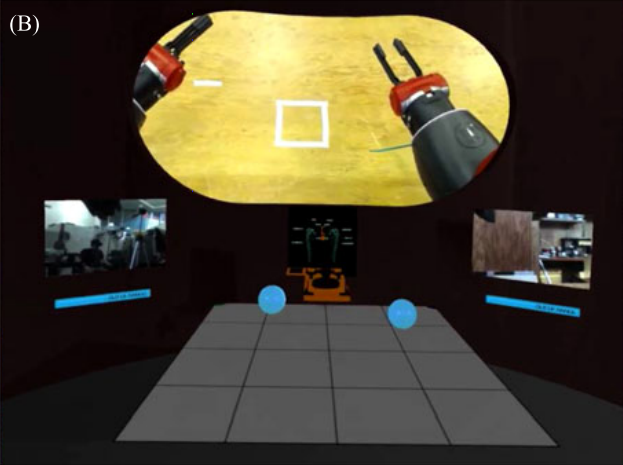
\includegraphics[width=0.45\textwidth]{Figures/homun.png} &
        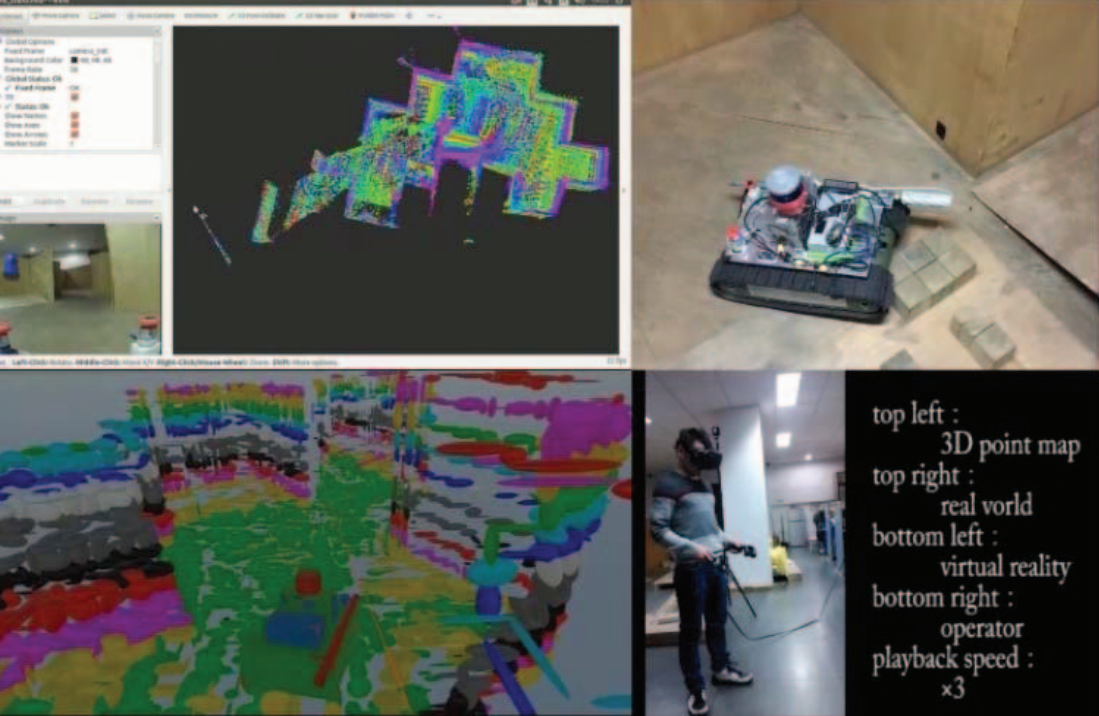
\includegraphics[width=0.5\textwidth]{Figures/lidar.png}
    \end{tabular}
    \caption[Indirect VR Teleoperations Examples]{Indirect VR Teleoperations Examples. A virtual control room based system (left) and a LiDAR 3D map based system (right), reproduced from \cite{lipton2018baxter} and \cite{wang2017novel}.}
    \label{fig:VRTele}
    \end{center}
\end{figure}

\section{Data Abstraction}
\label{Subsection:abstract}

\textit{Data abstraction} is the phrase that will be used in this report to describe the act of reducing an image down to only its most essential elements. It is similar in concept to an artist sketching a scene instead of attempting a full drawing. Comparing the concept to data compression is apt, as both aim to reduce the file size of the image, however data abstraction takes a very different approach to solving the problem than standard compression algorithms.

Data compression is the storing of information using a more space efficient encoding \cite{sayood2005introduction}. While some information is lost during lossy compression, the aim regardless of the algorithm used is to retain as much of the original information as possible. In contrast, the aim when utilising data abstraction is to discard all the information that is unnecessary to fulfilling the image's specific purpose. For example, if all that is required of an image is that basic shapes can be identified, then only the information on the boundaries of the shapes is necessary; the rest of the image can be discarded. An implementation of data abstraction can be seen in Figure \ref{fig:abstraction3rdyear}.

%\caption[My figure Title.]{My figure Title. Details how it was made. What is the point? Reproduced from}

\begin{figure}[H]
    \begin{center}
      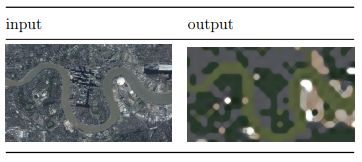
\includegraphics[width=0.6\textwidth]{Figures/abstraction3rdyear.png}
      \caption[Data Abstraction Example]{Data Abstraction Example. This is an abstraction of an aerial photograph of London, reproduced from \cite{abstraction3rdyear}.}
      \label{fig:abstraction3rdyear}
    \end{center}
\end{figure}

\section{Sobol Sequences}
\label{Subsection:sobol}

Sobol sequences are quasi-random sequences that were introduced to aid in approximating integrals. The aim is to form a sequence of points that are evenly spread across an S-dimensional unit cube \cite{joe2008constructing}, providing a much more even spread of points across the chosen space than can be produced from a pseudo-random number source (Figure \ref{fig:Sobol}). The code used in this project to produce these sequences was created by Leonhard Gr\"unschlo\ss\space \cite{CodeSource}.

\begin{figure}[H]
    \begin{center}
    \begin{tabular}{ c c }
        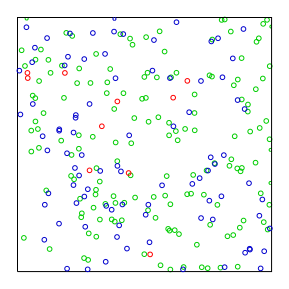
\includegraphics[width=0.33\textwidth]{Figures/Pseudorandom_sequence_2D.png} &
        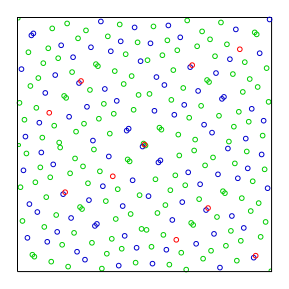
\includegraphics[width=0.33\textwidth]{Figures/Sobol_sequence_2D.png}
    \end{tabular}
    \caption[Comparison of Pseudo-Random and Quasi-Random Sequences]{Comparison of Pseudo-Random and Quasi-Random Sequences. 256 points from a pseudo-random generator (left) and 256 points from a Sobol sequence (right), reproduced from \cite{SobolWiki}.}
    \label{fig:Sobol}
    \end{center}
\end{figure}

\section{Computer Vision}

Computer vision is the automatic analysis of images and extraction of the useful information they contain \cite{CVDef}. A raw image is simply a large matrix of colour values, so for a computer to take action based on the contents of an image it must be able to recognise features using analysis of this data. Doing so involves a variety of techniques such as statistical pattern classification and geometric modelling \cite{ballard1982computer}. All computer vision methods in this project are implemented using the OpenCV libraries, and the example programs provided with them used as starting points for development \cite{OpenCV}.

\subsection{Edge Detection}
When attempting to recognise the features of an image, knowing the locations of the edges of objects within the scene is often valuable. An edge is defined as a significant local change in intensity, usually due to a discontinuity in either the intensity or its first derivative \cite{jain1995machine}. There are many algorithms available that will detect the edges of an image from the locations of these discontinuities. When the most popular algorithms (Laplacian of Gaussian, Robert, Prewitt, Sobel, and Canny) are compared \cite{maini2009study}, the most effective in almost all scenarios is Canny edge detection \cite{canny1986computational}, therefore this is the algorithm utilised in this project. Canny edge detection is demonstrated in Figure \ref{fig:canny1}.

\begin{figure}[H]
    \begin{center}
      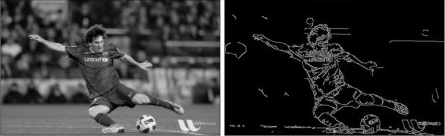
\includegraphics[width=0.9\textwidth]{Figures/canny2.png}
      \caption[Canny Edge Detection Example]{Canny Edge Detection Example. Simple edge detection program applied to a fairly detailed photo of Lionel Messi, to demonstrate its effectiveness with even complex images. Figure taken from an OpenCV edge detection tutorial \cite{Canny1Source}.}
      \label{fig:canny1}
    \end{center}
\end{figure}

\subsection{Flood Filling}

Flood fill algorithms determine the area connected to a given cell (the seed point) in a multi-dimensional array that have similar intensity values for the purpose of filling them with a chosen colour \cite{FloodFill}. This is a technique that is not only useful in image processing, but also for many other fields such as in passive acoustic monitoring, where finding the area connected to a given node can be useful as part of tracking in 4D space (x,y,z,time) \cite{nosal2008flood}. A demonstration of flood fill has been presented in Figure \ref{fig:EgFloodFill}.

\begin{figure}[H]
    \begin{center}
    \begin{tabular}{ c c }
        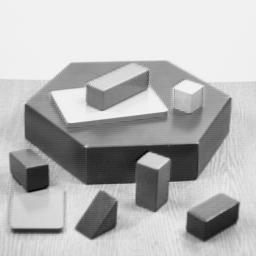
\includegraphics[width=0.35\textwidth]{Figures/blox.jpg} &
        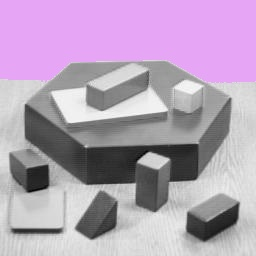
\includegraphics[width=0.35\textwidth]{Figures/bloxFilled.jpg}
    \end{tabular}
    \caption[Flood Filling Example]{Flood Filling Example. The original image (left) was provided by OpenCV \cite{OpenCV}. The right image is the result of flood filling from the top left corner.}
    \label{fig:EgFloodFill}
    \end{center}
\end{figure}

\subsection{Depth Mapping}
\label{subsection:depth}

The main component in the human brain's perception of 3D is the identification of disparity between the locations of objects in the 2D images being produced by its eyes \cite{qian1997binocular}. The greater the difference in the horizontal placement of an object between the images, the closer the object is to the observer. This technique can be used in computer vision to produce depth/disparity maps. Depth maps display differences in depth as a gradient from white to black (Figure \ref{fig:depthmap}), and can be produced using a variety of different algorithms. The most common are block matching algorithms, which use simple geometry and the matching of blocks of pixels horizontally in the 2 images to calculate depth \cite{linda2001stockman}. For these algorithms to locate the same object in different places in the 2 images, the cameras taking them must be calibrated to rectify any distortion due to the lenses \cite{distort} or discrepancies in the mounting that would cause them to be out of line \cite{stereocal}. Without this image rectification, the similar blocks the algorithm is attempting to locate will not be on the same horizontal row or will be distorted, so the algorithm will produce a mostly black image.

\begin{figure}[H]
    \begin{center}
      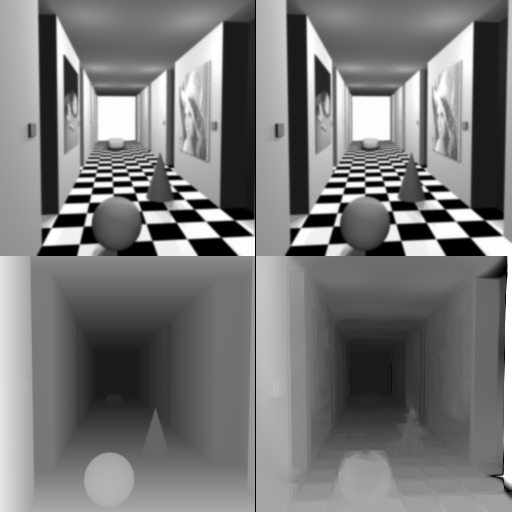
\includegraphics[width=0.8\textwidth]{Figures/depthmap.png}
      \caption[Depth Mapping Example]{Depth Mapping Example. A stereo pair of images, with their exact disparity map bottom left and a disparity map produced by a dense disparity estimation algorithm bottom right, reproduced from \cite{deptheg}.}
      \label{fig:depthmap}
    \end{center}
\end{figure} % Background 

\chapter{System Overview}
\lhead{\emph{System Overview}}
\label{chapter:system}

The telerobotics system presented consists of a fairly complex image processing pipeline running alongside a simple control system, with little interaction between the two (cf. Figure \ref{fig:system}). The pipeline starts with the two cameras on the rover taking a picture each as close to simultaneously as possible. These images then get abstracted down to edge detected sets of lines, with a set of colours also generated from \emph{Image 1} to combine with its edge detected version later on. These three pieces of data are then compressed into a single packet and transmitted via UDP \cite{postel1980user} to the server. The server splits them up again and produces a depth map from the two edge detected images. This depth map is passed to the 3D Environment to be used to produce a 3D model of the space the cameras were looking at. The server also combines the \emph{Colour Data} and \emph{Edge Detected Image 1} into a full coloured abstraction, which is overlaid onto the 3D model in the 3D environment. This environment is finally observed in the VR Headset.

The rover is controlled from an Xbox 360 controller \cite{360pad} that is connected to the server. Control inputs for driving the rover, gimble orientation, and parameters for the data abstraction (the only crossover between the control and image processing components) are transmitted to the rover at a fixed rate over UDP. It should be noted that in this system there is no connection between the orientation of the headset and gimble. The focus of this project was on providing the image processing foundations for future high presence systems, therefore the control system is the minimum required to explore the effectiveness of the chosen approach.

\begin{figure}[H]
    \begin{center}
      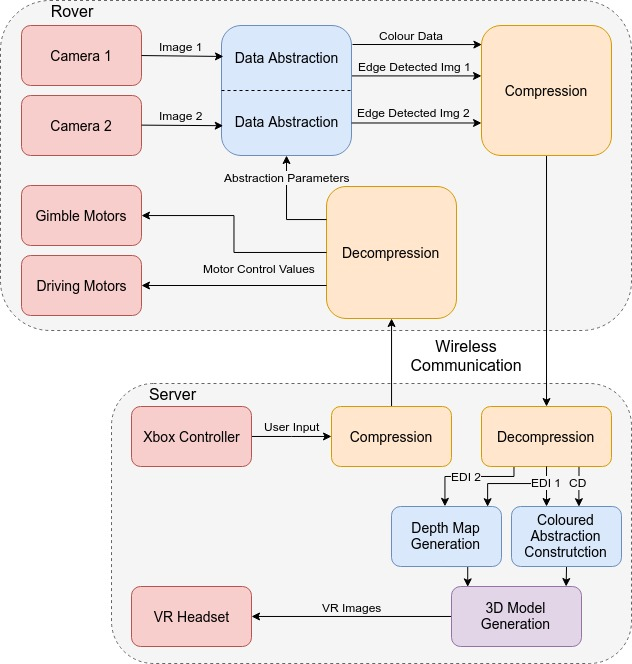
\includegraphics[width=0.8\textwidth]{Figures/System.jpg}
      \caption[System Overview Block Diagram]{System Overview Block Diagram. The red blocks represent input/output, the blue blocks represent image processing steps, the yellow blocks represent communications, and the purple block represents the 3D environment.}
      \label{fig:system}
    \end{center}
\end{figure} % System Overview

\chapter{Abstraction Algorithm Development}
\lhead{\emph{Abstraction Algorithm Development}}
\label{chapter:abstract}

In this implementation of data abstraction, the aim is to reduce images down to only the boundaries of the objects in the scene and then fill the spaces between theses boundaries with block colours based on the original image. Therefore the general process of the design is:
\begin{enumerate}
    \item Use edge detection on the image, presenting the boundaries of the scene as white lines and the rest as black. 
    \item Divide up the original image into sections that can reasonably be averaged into a single colour, defined by the boundaries produced by the edge detection or otherwise.
    \item Find the average colours (or reasonable alternatives) for these sections.
    \item Flood fill the spaces in the edge detection output with the average colours of the original image.
\end{enumerate}
While this section will be presented in the context of the entire process occurring on a single computer, when incorporated into the final system points 1-3 are implemented on the rover and point 4 is implemented on the server ("Coloured Abstraction Constrution" on Figure \ref{fig:system}). It is also worth noting that this chapter is concerned with the algorithm's ability to produce recognisable abstractions under reasonable resource constraints- the file sizes it is capable of producing will be covered as part of the discussion of the full system's communications protocol later on in Section \ref{Subsection:comms}.

\section{Edge Detection}

Canny edge detection was implemented using the Canny function provided by OpenCV. The sequence of processes implemented to support the algorithm in producing high quality edges are shown in Figure \ref{fig:CannyProc}. 

\begin{figure}[H]
    \begin{center}
    \begin{tabular}{ c c c }
        (1) & (2) & (3) \\
        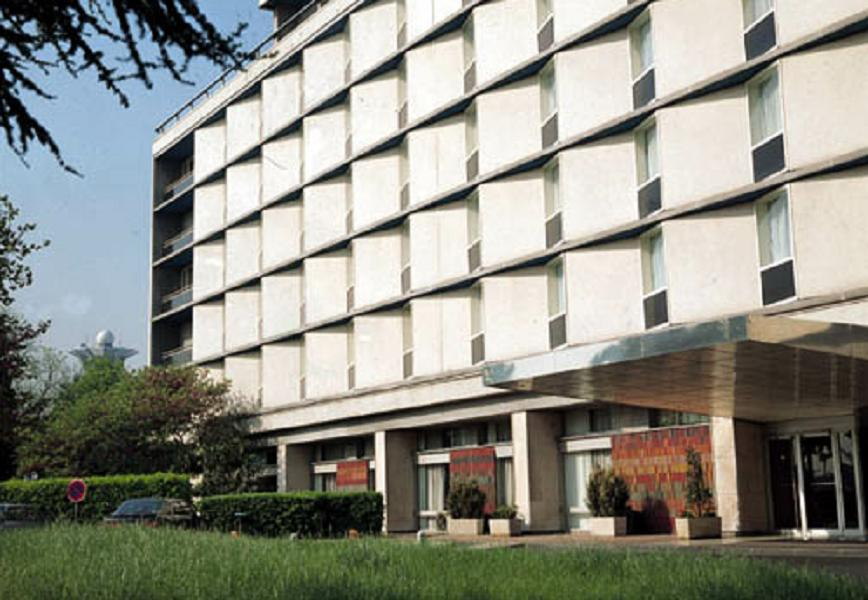
\includegraphics[width=0.31\textwidth]{Figures/building.jpg} &
        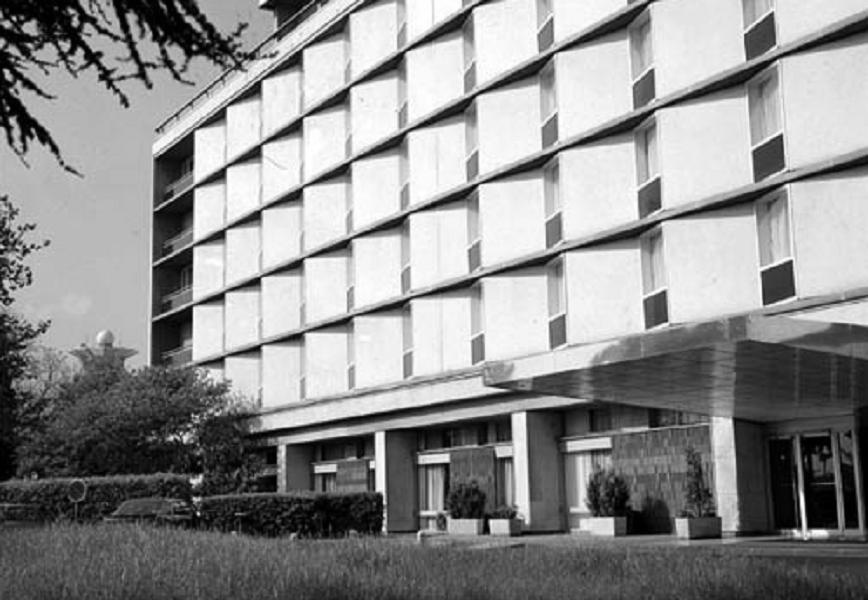
\includegraphics[width=0.31\textwidth]{Figures/buildGray.jpg} &
        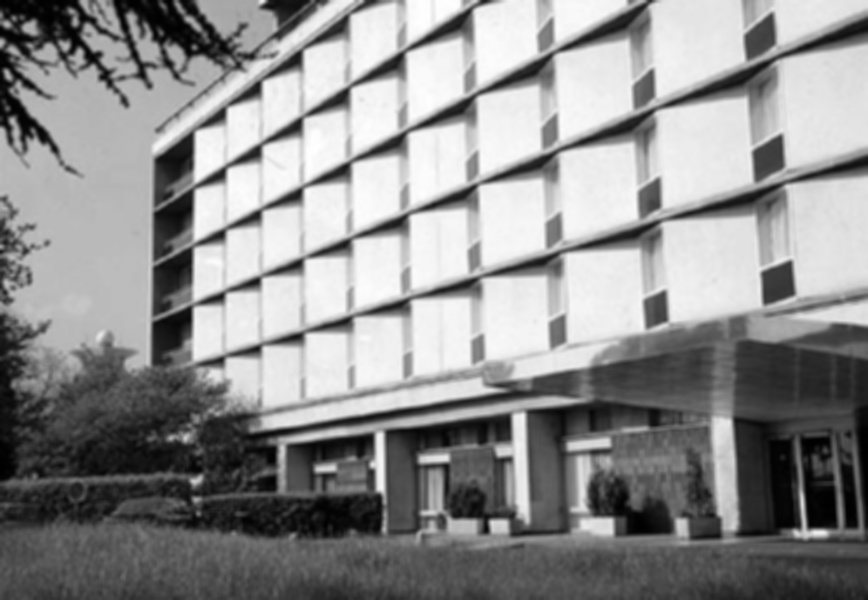
\includegraphics[width=0.31\textwidth]{Figures/buildBlur.jpg}
    \end{tabular}
    \begin{tabular}{ c c }
        (4) & (5) \\
        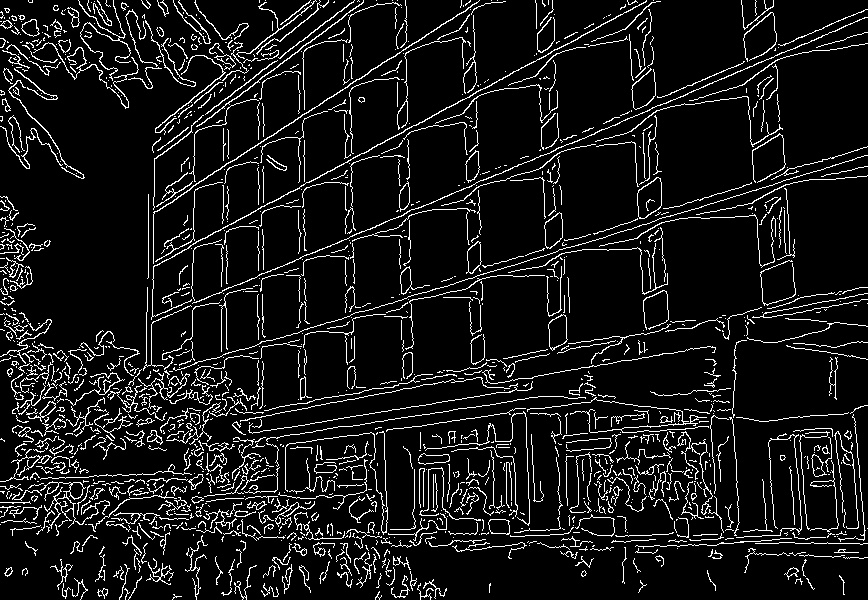
\includegraphics[width=0.31\textwidth]{Figures/buildCanny.jpg} &
        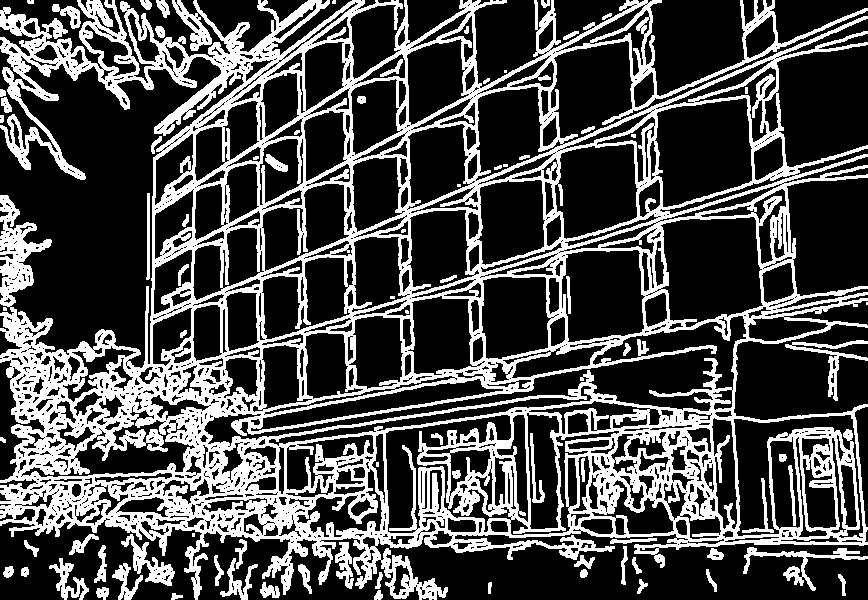
\includegraphics[width=0.31\textwidth]{Figures/buildDilated.jpg}
    \end{tabular}
    \caption[Process of Edge Detection]{(1) the original image, provided by OpenCV, (2) post grayscaling, (3) post blurring, (4) post edge detection, and (5) post dilation.}
    \label{fig:CannyProc}
    \end{center}
\end{figure}

The image is first made grayscale, as Canny detects large changes in light intensity and not colour. The image is then blurred to remove any unnecessary edges and noise that Canny may pick up. The edge detection is applied, producing white lines, representing the edges, on a black background. The output of the edge detection is finally dilated to make the lines thicker and bridge the gaps between the lines that are very close together. This is done to make the image more cartoon-like and more generally aesthetically pleasing, reduce the number of lines produced by areas that are dense with detail such as hair and foliage, and to bridge the gaps between lines that are close together, increasing the likelihood of defined shapes being created that can be easily flood filled later.

\section{Flood Filling}

Flood filling was chosen as the method for applying colour to the Canny output image, as it is an effective method for fill spaces of unknown size and shape that are defined by high contrast boundaries; using it makes dividing up the image into sections unnecessary. To use the OpenCV flood fill function you must provide a seed point to start flooding from, a colour to fill with, and parameters for the filling itself (unchanged from the defaults provided by the OpenCV documentation \cite{opencvffilldemo}).

\subsection{Seed Point}

Finding the points to flood fill from is a challenge, as each image will have a different number of spaces to be filled and the spaces can be anywhere. Three different methods were attempted to solve the problem. The first was an attempt to use OpenCV's contour functionality to turn the lines into a set of contours and use the centre of mass of each contour as the seed point. However, this was unusable due to high resource requirements. The method is detailed in Appendix C.

Although it would by ideal to aim to flood fill from the centre point of each space, it is only necessary if you intend to be selective about which pixels are being used as seed points.. It is possible to instead iterate through the whole image and flood fill from every pixel found that is not part of a line or an already filled space. This method is more effective at filling every space than the previous, and is also less resource intensive. However, if presented with a complicated environment with many spaces to flood fill it must fill every single one, leading to unacceptable drops in frame rate.

A simple solution to the performance issues caused by complex images would be to set a maximum number of times flood fill can be used per image. However, if this is done the seed points can no longer be selected by iterating through the whole image, as the presence of many small spaces at the top of an image would lead to larger, more important spaces not being filled at the bottom. The solution is to select a set number of points quasi-randomly across the image using Sobol sequencing (explained in Section \ref{Subsection:sobol}). Although a certain number of points will land on lines and therefore not be used, if there are enough points then all the important spaces are filled without serious impact on performance. Also, with this method performance is not affected by the complexity of the image, however more complicated images will be processed with many of the more dense areas unfilled (Figure \ref{fig:BrutevsSobol}). For these reasons, the seed points are selected using this method in the current build.

\begin{figure}[H]
    \begin{center}
    \begin{tabular}{ c c }
        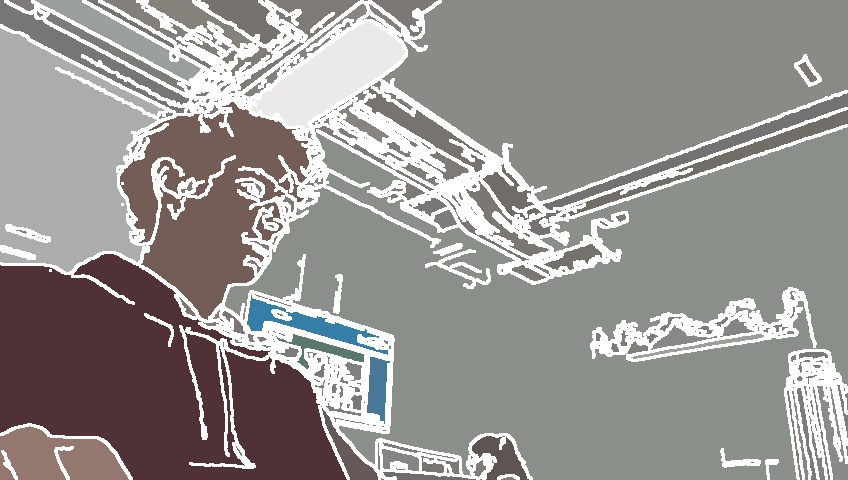
\includegraphics[width=0.45\textwidth]{Figures/Brute.jpg} &
        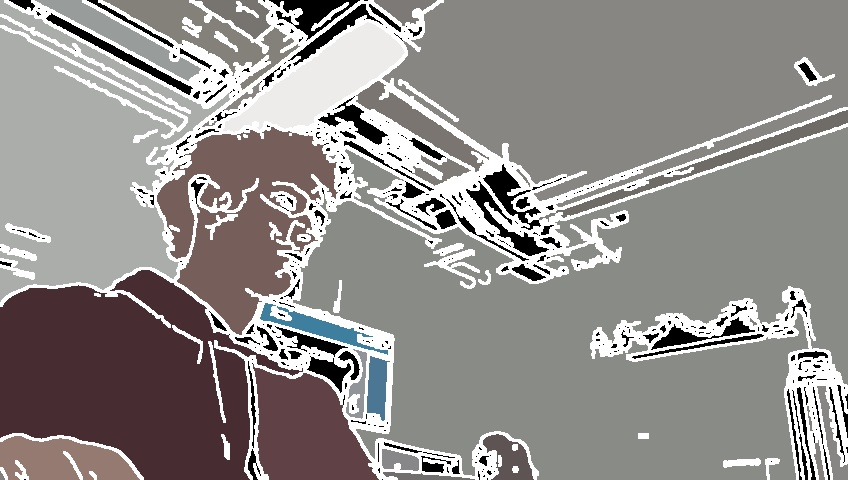
\includegraphics[width=0.45\textwidth]{Figures/Sobol.jpg}
    \end{tabular}
    \caption[Comparison of brute force and Sobol seed point generation]{Comparison of brute force and Sobol seed point generation. It can be clearly seen that the brute force method (left) accurately fills every space in the image, whereas using Sobol results in many unfilled spaces. However, Sobol is higher performance with a frame rate of 17.14fps, compared to 8.57fps using brute force.\textcolor{red}{[REDO FPS TESTS]}}
    \label{fig:BrutevsSobol}
    \end{center}
\end{figure}

\subsection{Fill Colour}

Three different methods were considered for finding the colours that the Canny output should be flood filled with. All three methods are valid solutions, but present different ratios between accuracy and resource requirements.

While filling the abstracted image with the average colours present within the input is preferable, it is not essential to the project; provided that the objects in the scene are still recognisable, they don't have to be exactly the right colour. For this reason it would be acceptable to not find the average colour of the area being flood filled at all, and instead simply use the colour of the seed point. This is a very fast method, however produces incredibly inconsistent colours between images. This is because there can be a wide spectrum of colour across a single surface even within the threshold of Canny edge detection, and the Sobol sequence will sample from a different point each time producing spaces that flicker between a wide range of colours.

The consistency of the previous method can be improved substantially with minimal impact on performance by taking an average of the colour within the area of a small circle around the seed point, rather than just the colour of that one point. This significantly improves the consistency between images, however introduces the problem of incorporating pixels from outside the space to be filled. This is due to the quasi-random points often being so close to the edge of the space that the averaging circle crosses the edge slighty and averages using part of a neighboring space. Therefore, the size of the circle must be carefully selected to balance the benefits of increasing size (more consistency when the seed point is further from the edge) and the benefits of decreasing size (more consistency when the seed point is closer to the edge). 

The OpenCV flood fill function provides the ability to fill a blank mask using the boundaries defined by a different image \cite{bradski2008learning}. This makes it possible to create a custom mask with the exact size and shape of the space that is to be filled and use that to find the average colour instead of the predefined circle. This produces the average colour of every space in the image exactly at the expense of adding an extra stage of flood filling before the Canny output itself is filled (a stage of flood filling that would have to be undertaken on the rover in the full system). The consistency between images for this is the maximum possible based on colour alone (Figure \ref{fig:ColourConsistency}), though inconsistency in the edge detection causes certain spaces to combine and divide constantly, leading to a small amount of colour inconsistency to remain regardless. This method has a noticeable impact on performance, though within acceptable bounds \textcolor{red}{[DATA?]}, leading this to be the chosen method to be implemented into the full system. Examples of the results produced by the final single computer based build can be seen in Appendix D.

\begin{figure}[H]
    \begin{center}
      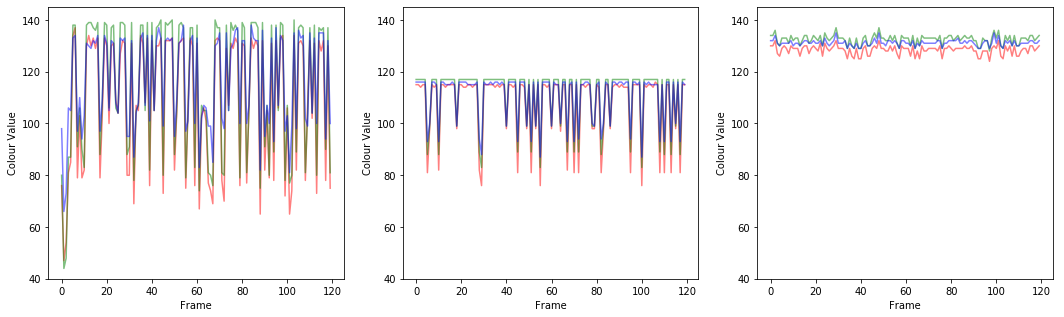
\includegraphics[width=1\textwidth]{Figures/ColourConsistency.png}
      \caption[Comparison of Colour Averaging Methods]{Comparison of Colour Averaging Methods. These are RGB values over time produced by flood filling an example area using the seed point colour (left), circle average (middle), and flood fill average (right). The increase in consistency from left to right is very apparent.}
      \label{fig:ColourConsistency}
    \end{center}
\end{figure} % Abstraction Algorithm Development

\chapter{Rover Implementation}
\lhead{\emph{Rover Implementation}}
\label{chapter:rover}

Due to the rover's purpose being to provide a simple test platform for a teleoperations system, its hardware is fairly simple. The motor drivers and motors used to turn the rover's wheels are located internally alongside the batteries and power distribution board, while the central computer (Raspberry Pi 3 \cite{pi}), gimbal, and gimbal control circuitry are all mounted on the top of the chassis (Figure \ref{fig:internals}, \ref{fig:hardware}). A detailed breakdown can also be found in Appendix \ref{appendix:hardware}. The application of computer vision techniques in an embedded system has high processing requirements, leading to the selection of a Raspberry Pi 3 as the core of the system (it was the highest performance embedded device readily available). 

\begin{figure}[H]
    \begin{center}
    \begin{tabular}{ c }
        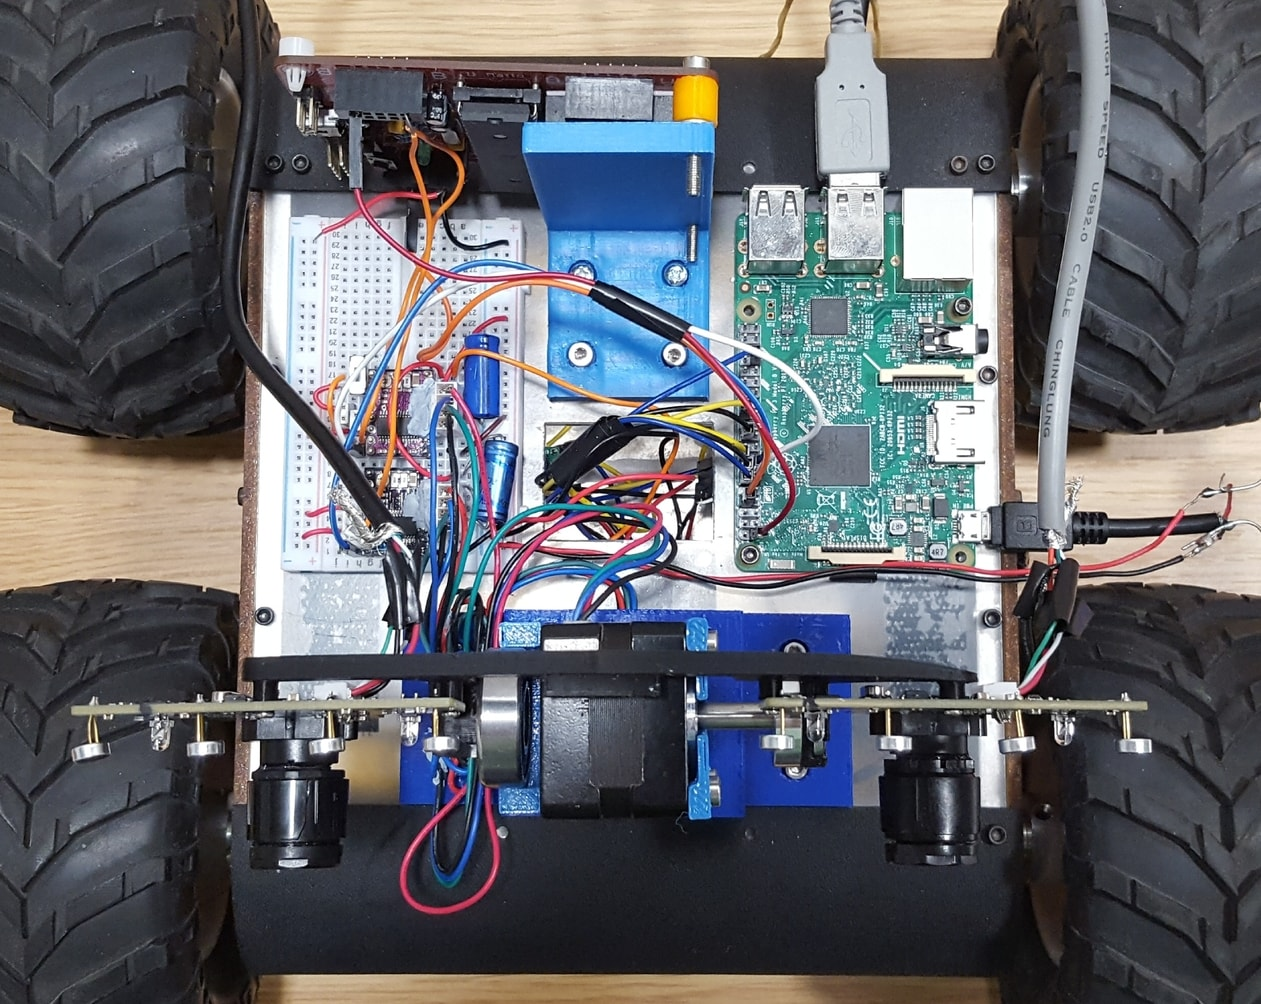
\includegraphics[width=0.75\textwidth]{Figures/rovertop.jpg} \\
        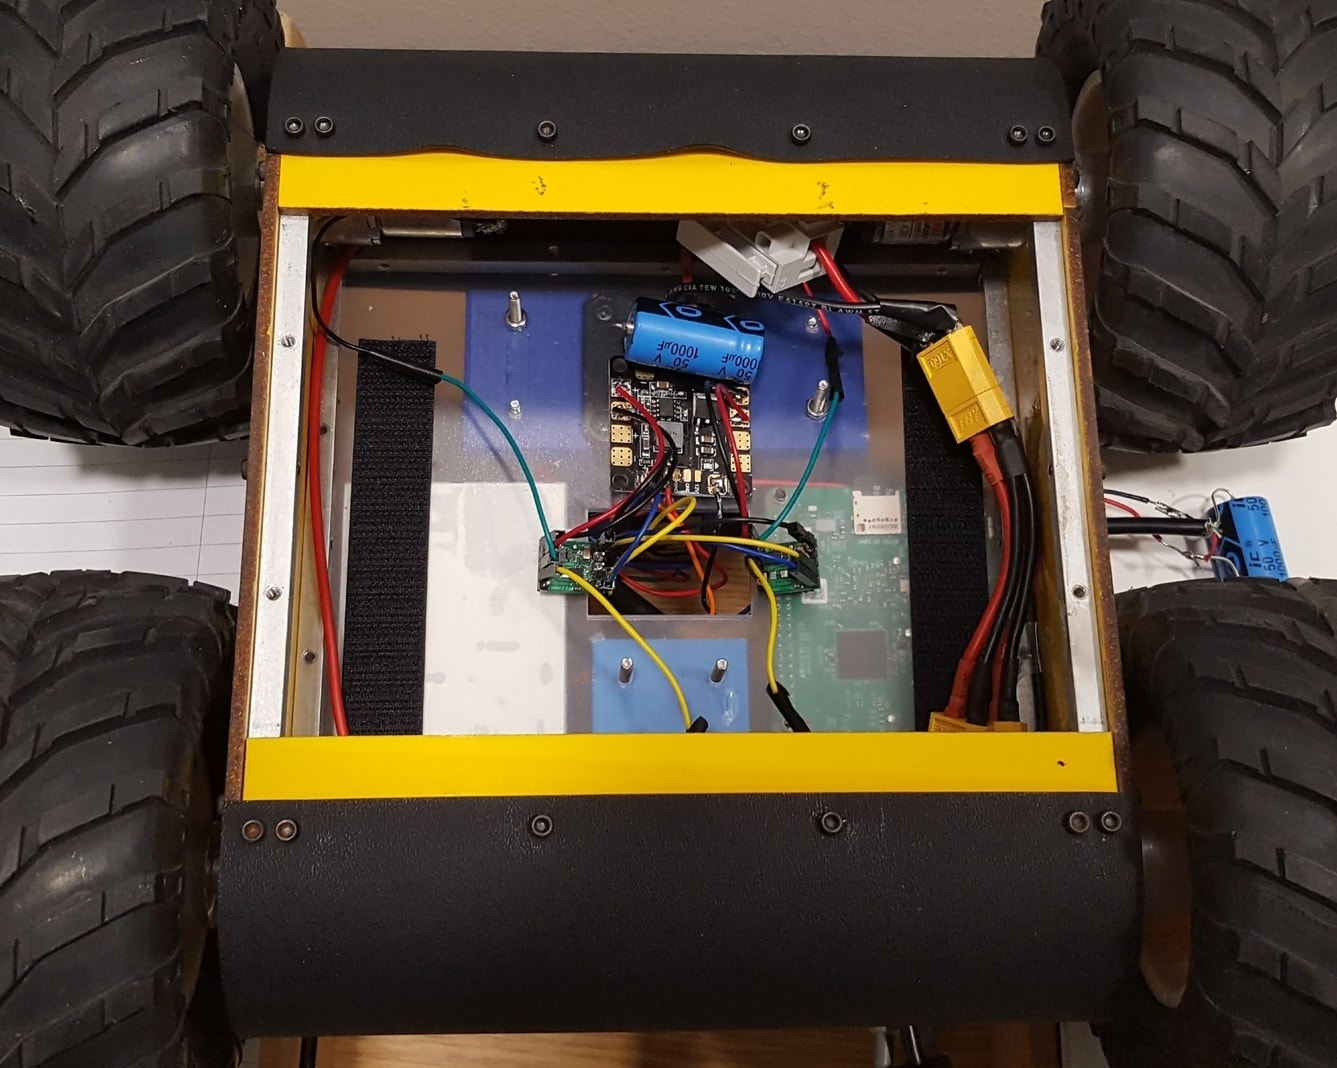
\includegraphics[width=0.75\textwidth]{Figures/roverinside.jpg}
    \end{tabular}
    \caption[Rover Internals]{Rover Internals. The left picture is a top-down view of rover, in which you can see the Pi on the right, the Il Matto mounted vertically at the top, the gimbal at the bottom, and the stepper motor drivers for the gimbal on the breadboard on the left. The right picture is of the inside of the rover, taken through a hatch in its underside. In this picture you can see velcro strips marking where the batteries are attached, a power distribution board and fuse in the centre, 2 DC motor drivers just below that, and 2 of the 4 DC motors in the top corners.}
    \label{fig:internals}
    \end{center}
\end{figure}

\begin{figure}[H]
    \begin{center}
      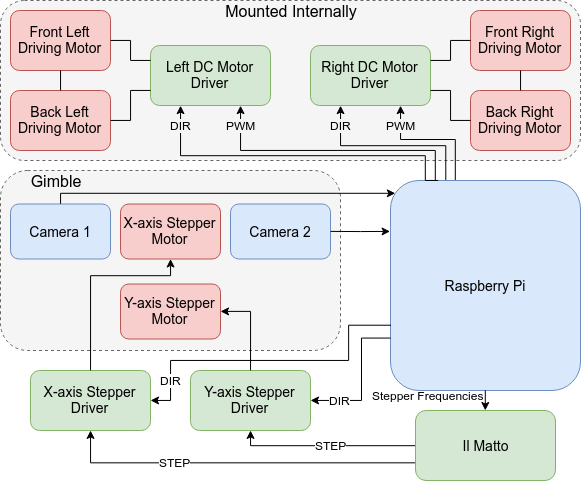
\includegraphics[width=0.9\textwidth]{Figures/hardware.png}
      \caption[Hardware Block Diagram]{Hardware Block Diagram. The red blocks are motors, green blocks are control system components, and the blue blocks are part of the image pipeline.}
      \label{fig:hardware}
    \end{center}
\end{figure}

\section{Gimbal Design}

The choice of cameras had to fulfil a very specific set of requirements. The two cameras must be same, as any differences in the images due to the cameras would reduce the quality of depth map produced by the block matching algorithm on the server. This makes the most obvious camera choice, the R-Pi camera module, unusable, as the Pi cannot use two simultaneously. The two cameras must also be able to take pictures on command from the Pi with low latency, reducing the possible options down to primarily USB webcams. Finally, they must have a high shutter speed. Any motion blur in the images will blur all the edges they contain, making them undetectable by the edge detection algorithm, and any morphing of the image while under motion due to the time it takes the shutter to pass across the entire sensor will once again reduce the quality of the depth map; a high shutter speed reduces motion blur and shutter related morphing, therefore making it essential for whenever the rover is in motion. This requirement reduces the possible cameras down to primarily dedicated computer vision cameras, however these are far outside the budget of a 3rd year project and are often too large to build a gimbal for without also buying expensive motors.

Only one camera was found that fulfilled all these requirements whilst also being reasonably priced- the PlayStation 3 (PS3) Eye. The PS3 Eye is a peripheral for the PS3 that facilitates games that incorporate aspects of computer vision, so it is designed with computer vision and value for money in mind. While the image quality is fairly poor, this does not significantly impact the quality of abstractions the system produces. The only real flaw in using the PS3 Eye in this system is its poor dynamic range; if the camera is aimed at a window during the day, all the colours in the room will become unrecognisably dark. However, the fast shutter speed and low latency more than make up for this deficiency.

The design of the gimbal (Figure \ref{fig:gimble}) has considerable impact on the 3D model the system generates. As mentioned in Section \ref{subsection:depth}, the closer the cameras are to parallel with each other, the less the images have to be rectified before the depth map is generated. Similarly, the stability of the gimbal is very important, as any vibrations will cause inconsistency in the alignment of the cameras, leading to inaccurate depth maps. This led to the chosen design where the X-axis (tilt) motor is located centrally, between the cameras, to balance the weight around the rotational axis of the y-axis (rotation) motor. The 3D-printed part the cameras are attached to is also stabilised through mountings on both sides of the x-axis motor, using a ball bearing on the side not driven by the motor. 

\begin{figure}[H]
    \begin{center}
      \includegraphics[width=0.75\textwidth]{Figures/gimble.jpg}
      \caption[Gimbal Picture]{Gimbal Picture. The Y-axis motor is housed at the bottom, with the X-axis motor directly above it. The ball bearing that stabilises the non-driven side of the cameras' backplate can be seen to the left of the X-axis motor.}
      \label{fig:gimble}
    \end{center}
\end{figure}

Another important aspect of the gimbal design is the distance between the camera lenses. The further apart the two cameras are, the closer distance objects will be in the depth map. Ideally we would want to match the interpupillary distance of human eyes (63mm on average \cite{dodgson2004variation}), so objects in the 3D environment appear as close as they would were the user standing in the place of the robot. However, with the X-axis motor located centrally, it is not possible to produce that distance between the camera lenses. The inter-lens distance in the final design is 120mm, as this is the closest distance possible without reducing the stability of the gimbal. While not ideal, it simply results in objects appearing closer in the depth map than they actually are and a longer distance from the cameras where an object is too close for a distance to be calculated (the cameras are "cross-eyed" if you will).

\section{Image Pipeline}
\label{Subsection:comms}

As can be seen in Figure \ref{fig:system}, the rover takes a picture with both cameras, abstracts those images, then sends that data off as a single combined packet to the server. While Chapter \ref{chapter:abstract} discussed the abstraction process as a single step that produces a full abstraction with both edges and spaces filled with colour, this does not reflect the implementation utilized in the full system. As previously mentioned, the final step of filling the spaces in the edge detected image using the selected seed points and average colours is done on the server. Also, only one of the two images needs colour information at all, as the edges are the only part of the abstraction required to produce the server depth maps; the colours are to be used as a texture on the 3D environment this produces, and therefore only one set is required. Therefore, the data packets being sent to the server are made up of 2 bitmaps of the edge detected images and a set of seed points with their corresponding colours for one of the images.

Attempts to implement this process on a single thread on the Pi, as tested successfully on a laptop, either crashed the Pi or would produce an unacceptable frame rate of around 1fps. To rectify this, both pipelining and parallelism were utilized to make better use of the Pi's quad core processor (Figure \ref{fig:threads}), and compromises were made in the quality of the abstractions to reduce the workload.

\begin{figure}[H]
    \begin{center}
      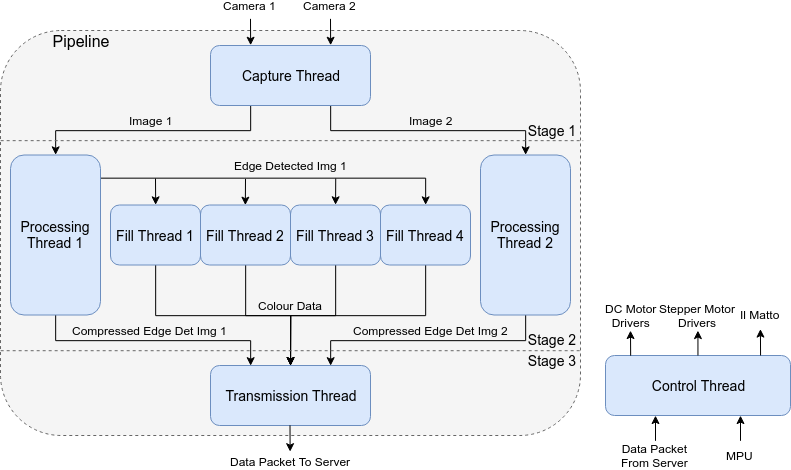
\includegraphics[width=0.9\textwidth]{Figures/Threads.png}
      \caption[Raspberry Pi Image Pipeline Threading Block Diagram]{Raspberry Pi Image Pipeline Threading Block Diagram.}
      \label{fig:threads}
    \end{center}
\end{figure}

The capture thread simply handles signalling the cameras to take a picture each. The capture and decoding of the images are done as separate operations to make the capture operation shorter and therefore the two cameras capturing as close to simultaneously as possible with a single thread. The first compromise in quality in favour of performance is made here, where the images are captured with a resolution of 320x240 rather than the cameras' standard resolution of 640x480. As will be discussed in greater depth below, the highest workload task in the pipeline is flood filling. Reducing the pixel count of every space by a factor of four therefore provided a significant improvement in performance. The smaller images also have the benefit of lower detail in high detail areas, so sections that would become areas of dense lines when edge detected (examples of this effect can be found in Appendix \ref{Appendix:demo}) are significantly less dense, containing less extraneous data.

The processing threads are concerned with the edge detection and compression of the images. The edge detection process is mostly as described in Chapter \ref{chapter:abstract}; the only difference is only the image being sent from processing thread 1 to the fill threads undergoes the final dilation step. The purpose of the dilation is to bridge gaps between the edges, creating defined shapes for the flood fill process. A side effect of dilation is a reduction in edge accuracy, which is very important when the images are to be used to produce depth maps later on. This leads to the logical conclusion that the images should be sent without dilation, and dilation only applied to find the colour data in the fill threads and then again on the server to create the complete coloured abstraction, allowing the depth maps to be constructed with non-dilated images. 

While it can be induced from comparing the original images to their edge detected versions by eye that the latter contains less information than the former, this will only be reflected in real numbers if file format and compression are considered carefully. When the common image formats are compared, PNG would appear to be effective for this use case \cite{aguilera2006comparison}, as it excels at efficiently storing large blocks of the same colour (most of each edge detected image is black space). When tested on the edge detected images (Figure \textcolor{red}{[COMPRESSION COMPARISON]}), it was confirmed that PNG provided the lowest file size, and compression level 5 provided the best ratio between file size and compression time (using the imencode function in OpenCV). More intelligent compression was tested using libimagequant \cite{libimagequant}, however it resulted in very poor performance (\textless2fps) with negligible improvement to the level of compression. An alternate option to compression as a bitmap was vectorising the images, however this was inaccurate and not as effective as bitmap compression (more information can be found in Appendix \ref{appendix:vectorization}).

The stage in the image pipeline that has the highest performance impact is the colour averaging, due to its use of flood filling. As the number of spaces being flood filled is determined by the number of points from the sobol sequence being sampled, the number of sobol points is an important variable in tuning the performance of the system. In the testing done on a laptop in Chapter \ref{chapter:abstract}, the number of sobol points being used per image was always between 400 and 600, and this filled a reasonable number of spaces while providing a reasonable frame rate of around 15fps. When this was attempted on the Pi however, the frame rate was significantly below 1fps. This called for a significant reduction in sobol points and the application of parallelism; good performance was achieved using 4 threads dedicated to the flood fill colour averaging task, each taking 15 sobol points. A total of 60 sobol points is a significant reduction from the laptop implementation of the algorithm, however it must also be noted that the images being used are much smaller, so do not require a large number of sobol points to have been mostly covered (Figure \textcolor{red}{[ROVER/LAPTOP ABSTRACTION COMPARISON]}). While it may seem as though the parallelization of this process could cause issues if two threads are attempting to fill the same space in the image simultaneously, this simply results in two successful seed points with slightly inaccurate average colours assigned to them, and only one of them being used to create the complete abstraction on the server. As the colours of the spaces are only recorded to provide the user a better understanding of the objects in the environment, it is not concerning if occasionally one is not an exact average.

Once the three pieces of data for an image pair (two compressed edge detected images and a set of colour data) have been generated, they must be combined into a single packet and sent to the server; this is covered by the transmission thread. While the images are at this stage already compressed into a set of bytes that can be transmitted as is, the colour data needs its own custom packaging. Each seed point-average colour pair is formed into its own sub-packet with the structure shown in Table \ref{table:colour}. These sub-packets make up the colour data data segment within the complete data packet.

\begin{table}[H]
\centering
\caption{Colour Data Sub-Packet Structure. The seed point components are given 2 bytes each due to their maximum values being larger than a single byte can store.}
\label{table:colour}
\begin{tabular}{|c|c|c|c|c|c|c|c|}
\hline
Byte in Colour Data Sub-Packet & 1          & 2         & 3          & 4         & 5         & 6           & 7         \\ \hline
Usage                          & \multicolumn{4}{c|}{Seed Point}                 & \multicolumn{3}{c|}{Average Colour} \\ \hline
Component                      & \multicolumn{2}{c|}{X} & \multicolumn{2}{c|}{Y} & Red       & Green       & Blue      \\ \hline
\end{tabular}
\end{table}

As the size of each data segment is unknown and highly variable, knowing where one ends and another begins on the server is a challenge. The solution utilized in this instance is separating each data set with a splitter made up of 7 bytes that contain 0, 1, 2, 3, 4, 5, and 6. This sequence of bytes is extremely unlikely to occur within the data, so can be easily used to pinpoint the starts and ends of the data sets. This therefore leads to the data packet format shown in Table \ref{table:packet}.

\begin{table}[H]
\centering
\caption{Data Packet Format.}
\label{table:packet}
\resizebox{\textwidth}{!}{
\begin{tabular}{|c|c|c|c|c|c|c|c|}
\hline
Data Segment & \multicolumn{3}{c|}{Colour Data}  & Splitter & Img 1          & Splitter & Img 2          \\ \hline
Contents     & Sub-Packet 1 & Sub-Packet 2 & ... & 0...6    & PNG Data & 0...6    & PNG Data \\ \hline
\end{tabular}}
\end{table}

\section{Control System}

%Xbox controls

%Data packet format

The primary aim when designing the control system was to make controlling the rover easy and intuitive; the user must have no trouble understanding the controls whether in or out of VR. The obvious first consideration for the control input method is through a keyboard and mouse, as this is standard practice in teleoperations. However, operating a keyboard whilst in VR is very difficult, as the user must be able to see both their hands and the keyboard to know which keys they are pressing. A better direction would be to consider which input methods are standard use in VR gaming, as these are known to be intuitive without the user having visibility of their hands. The most common VR input methods are dedicated VR controllers, such as the Vive controllers, and standard gamepads, such as the Xbox 360 controller (Figure \textcolor{red}{[CONTROLLERS?]}). Due to being visible within the VR environment (they are tracked like the headset), the Vive controllers are the most intuitive method within VR, however they cannot be used outside VR, so do not facilitate testing the control system without an active VR headset connected. The Xbox controller is a great general use controller, as it can be integrated into almost anything and is intuitive at any stage of testing, leading it to be the chosen control input method.

The motion of the rover is restricted to forwards or backwards with variable speed, or rotation with a fixed speed. This is so the rover is forced to only rotate in short intervals, as rotation causes a reduction in depth map accuracy that forward and backwards motion does not (the extent and causes of this will be discussed in Chapter \ref{chapter:eval}). The user has the ability to chose between full and half speed drive modes, to provide the flexibility of both being able to run the motors at full power in one mode and drive at low speeds with greater control in the other. Due to the gimbal not having a full range of motion (it can rotate roughly 200 degrees before it starts to pull its own cabling out), its range must be restricted in software. This is done by keeping track of the number of steps the stepper motors have undertaken as an estimator of the gimbal's orientation, and preventing it from moving past certain angles. This system is effective, however the limits drift over time due to the stepper motors not always moving through the exact same number of steps requested by the control system. This drift, while not ideal, is only an issue over long activation periods, so is not a major concern for this project. The final element the user has control over is the low threshold in the edge detection applied as part of the data abstraction in the rover (this is the single point of contact between the image pipeline and control system that is mentioned in Chapter \ref{chapter:system}). Changing the threshold of the edge detection can have a major impact on the quality of the 3D model the system produces, and the ideal threshold changes depending on the space the rover is observing, therefore it is essential that the user has control of this at run-time.

The user inputs are transmitted to the rover over UDP, each packet with the structure shown in Table \ref{table:control}. The packets are sent at a constant rate of 50 per second, even when the user is not inputting any commands. This is so that the rover knows when the wireless link is failing, as that constant message stream will be inconsistent or stop entirely. When the rover detects that it has been an unreasonable amount of time since the last message, it stops all its motors until it starts receiving messages again, to prevent it from damaging itself while the user has lost control.

\begin{table}[H]
\centering
\caption{Control Data Packet Structure. The analogue stick axes are mapped to between 0 and 255 to fit them within a byte each, as greater accuracy than that was not required. The low threshold only being alocated a byte means it is also capped at 255, however through testing it has been determined that values even above 100 produce images with no edges anyway, so this limit is not a concern.}
\label{table:control}
\resizebox{\textwidth}{!}{
\begin{tabular}{|c|c|c|c|c|c|c|}
\hline
Byte in Control Packet & 0                                                 & 1                                                & 2               & 3                                                 & 4                                                & 5          \\ \hline
Usage                  & \multicolumn{2}{c|}{\begin{tabular}[c]{@{}c@{}}Driving Control\\ (Left Analogue Stick)\end{tabular}} & Low Threshold   & \multicolumn{2}{c|}{\begin{tabular}[c]{@{}c@{}}Gimbal Control\\ (Right Analogue Stick)\end{tabular}} & Drive Mode \\ \hline
Contents               & X-axis                                            & Y-axis                                           & Threshold Value & X-axis                                            & Y-axis                                           & 0/1        \\ \hline
\end{tabular}}
\end{table} % Rover Implementation

\chapter{Server-Side Implementation}
\lhead{\emph{Server-Side Implementation}}
\label{chapter:server}

%Relation to gimble position

The purpose of the server is to receive image data from the rover, produce a 3D environment from it, and feed back control inputs from the user. This is all done within the framework of the 3D game engine Unreal Engine 4 \cite{unreal}. Unreal 4 was chosen because it provides easy interfacing with almost any VR headset on the market without large rewrites of the code, it is simple to integrate with OpenCV, and is free to use.

\section{Depth Mapping}

\section{Coloured Abstraction Construction}

As previously established, to produce the final texture that is applied to the 3D environment, a complete coloured abstraction must be produced from the dominant camera image and colour data.

\section{3D Environment Generation}

 % Server-Side Implementation

\chapter{Project Evaluation and Conclusion}
\lhead{\emph{Project Evaluation and Conclusion}}

%Comparison of product and brief
%Evaluation of project management
%Conclusion

\chapter{Project Management}
\lhead{\emph{Project Management}}
\label{chapter:mang}

Comparison of product and brief
Evaluation of project management

\chapter{Conclusion}
\lhead{\emph{Conclusion}}
\label{chapter:conclusion}

The aim of this project was to research the use of data abstraction to minimise the technical issues involved with VR telerobotics through the design and implementation of an abstraction based teleoperations system. Through its use of a 3D model, the system created does not cause motion sickness when operated, successfully mitigating the primary issue with VR telerobotics. The 3D model updates at 20-25 fps with a latency of 0.25-0.5 seconds, providing the user reasonably responsive controls, and is also accurate enough to provide the user spacial awareness. The novel data abstraction algorithm implemented allows this to be achieved with data packets of $<$8kB each.

The next steps for this research would be to replace the R-Pi with a more powerful alternative, with the aim of mitigating the issues with the system that are linked to the R-Pi's bottlenecking, and to improve the system's ability to represent slanted surfaces. As the depth information required to correctly map a slanted surface is already present in the edge detected images of it, it is the depth mapping and depth map filtering that must be redesigned to better extract that information.

\addtocontents{toc}{\vspace{2em}}  % Add a gap in the Contents, for aesthetics
%\backmatter
%% ----------------------------------------------------------------
\label{Bibliography}
\lhead{\emph{Bibliography}}  % Change the left side page header to "Bibliography"
\bibliographystyle{ieeetr}  % Use the "unsrtnat" BibTeX style for formatting the Bibliography
\bibliography{Bibliography}  % The references (bibliography) information are stored in the file named "Bibliography.bib"
\addcontentsline{toc}{chapter}{Bibliography}

%% ----------------------------------------------------------------
% Now begin the Appendices, including them as separate files

\addtocontents{toc}{\vspace{2em}} % Add a gap in the Contents, for aesthetics

\appendix % Cue to tell LaTeX that the following 'chapters' are Appendices

\chapter{Demonstrations of Full Data Abstraction}
\lhead{\emph{Demonstrations of Full Data Abstraction}}

\begin{figure}[h]
    \begin{center}
    \begin{tabular}{ c c }
        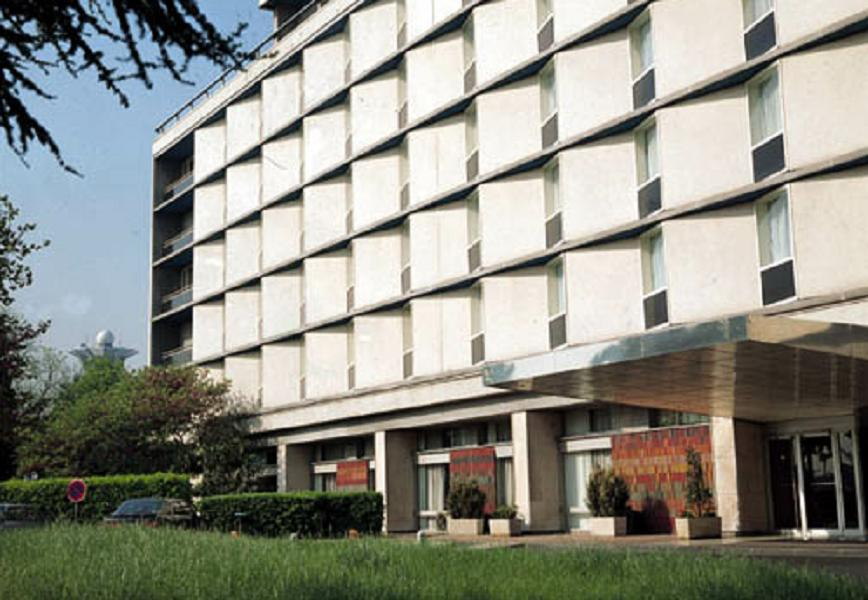
\includegraphics[width=0.45\textwidth]{Figures/building.jpg} &
        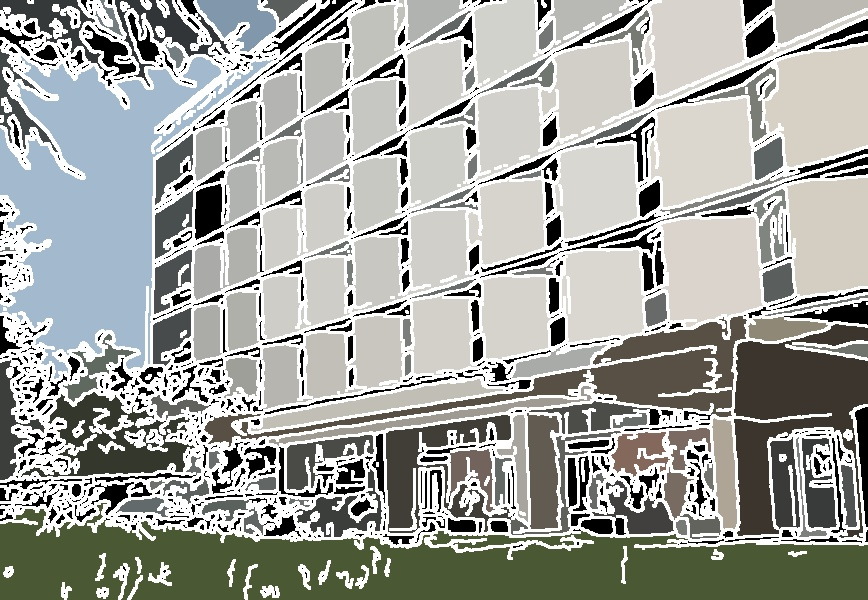
\includegraphics[width=0.45\textwidth]{Figures/Final.jpg} \\
    \end{tabular}
    \caption[Demonstration of full abstraction process]{Demonstration of full abstraction process. The final parameters and methods (of those under discussion) are a blur kernel of 5x5, a low threshold of 25 (for this example), Sobol seed point generation, and averaging via preliminary flood fill. It can be seen that most areas of the image are being effectively edge detected and flood filled with the correct colours; however, some areas are hard to interpret such as around the bushes in the bottom left, and some spaces have been left unfilled such as the panel below the top left corner of the building. These issues are minimal though, therefore leading me to conclude that the process is effective at producing recognisable abstractions of the input images.}
    \label{fig:Final}
    \end{center}
\end{figure}
        
\begin{figure}[h]
    \begin{center}
    \begin{tabular}{ c c }
        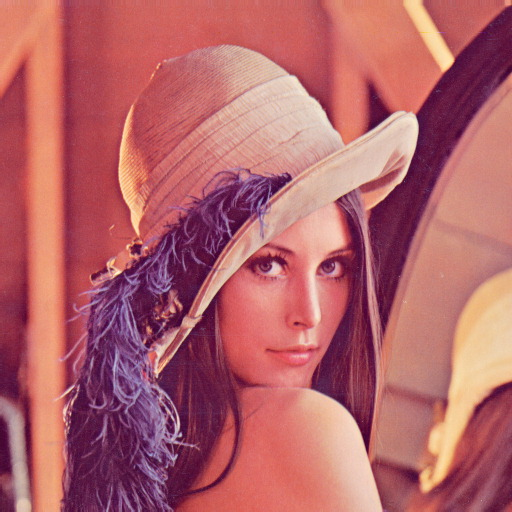
\includegraphics[width=0.45\textwidth]{Figures/lena.jpg} &
        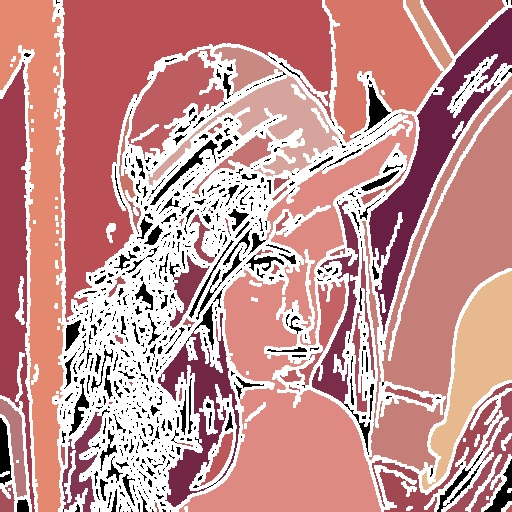
\includegraphics[width=0.45\textwidth]{Figures/lenaDA.jpg} \\
        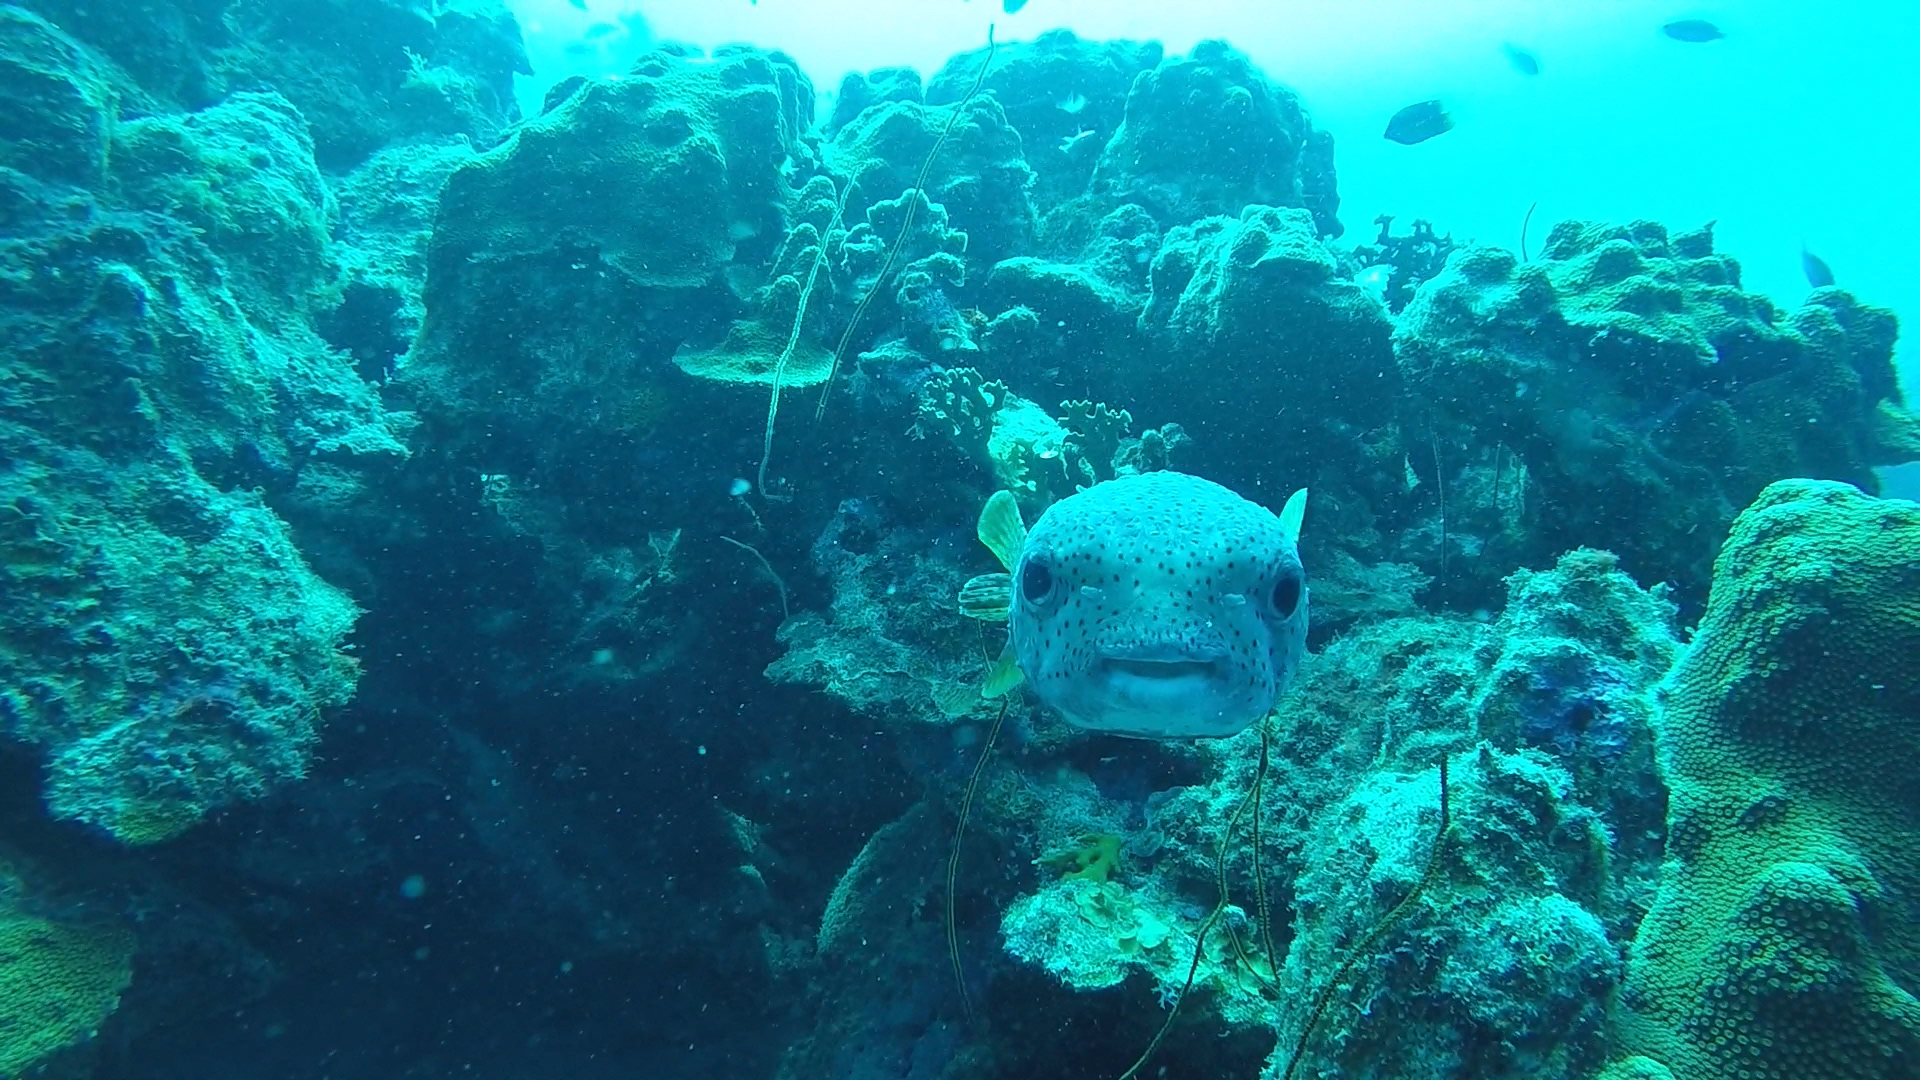
\includegraphics[width=0.45\textwidth]{Figures/pufferfish6.jpg} &
        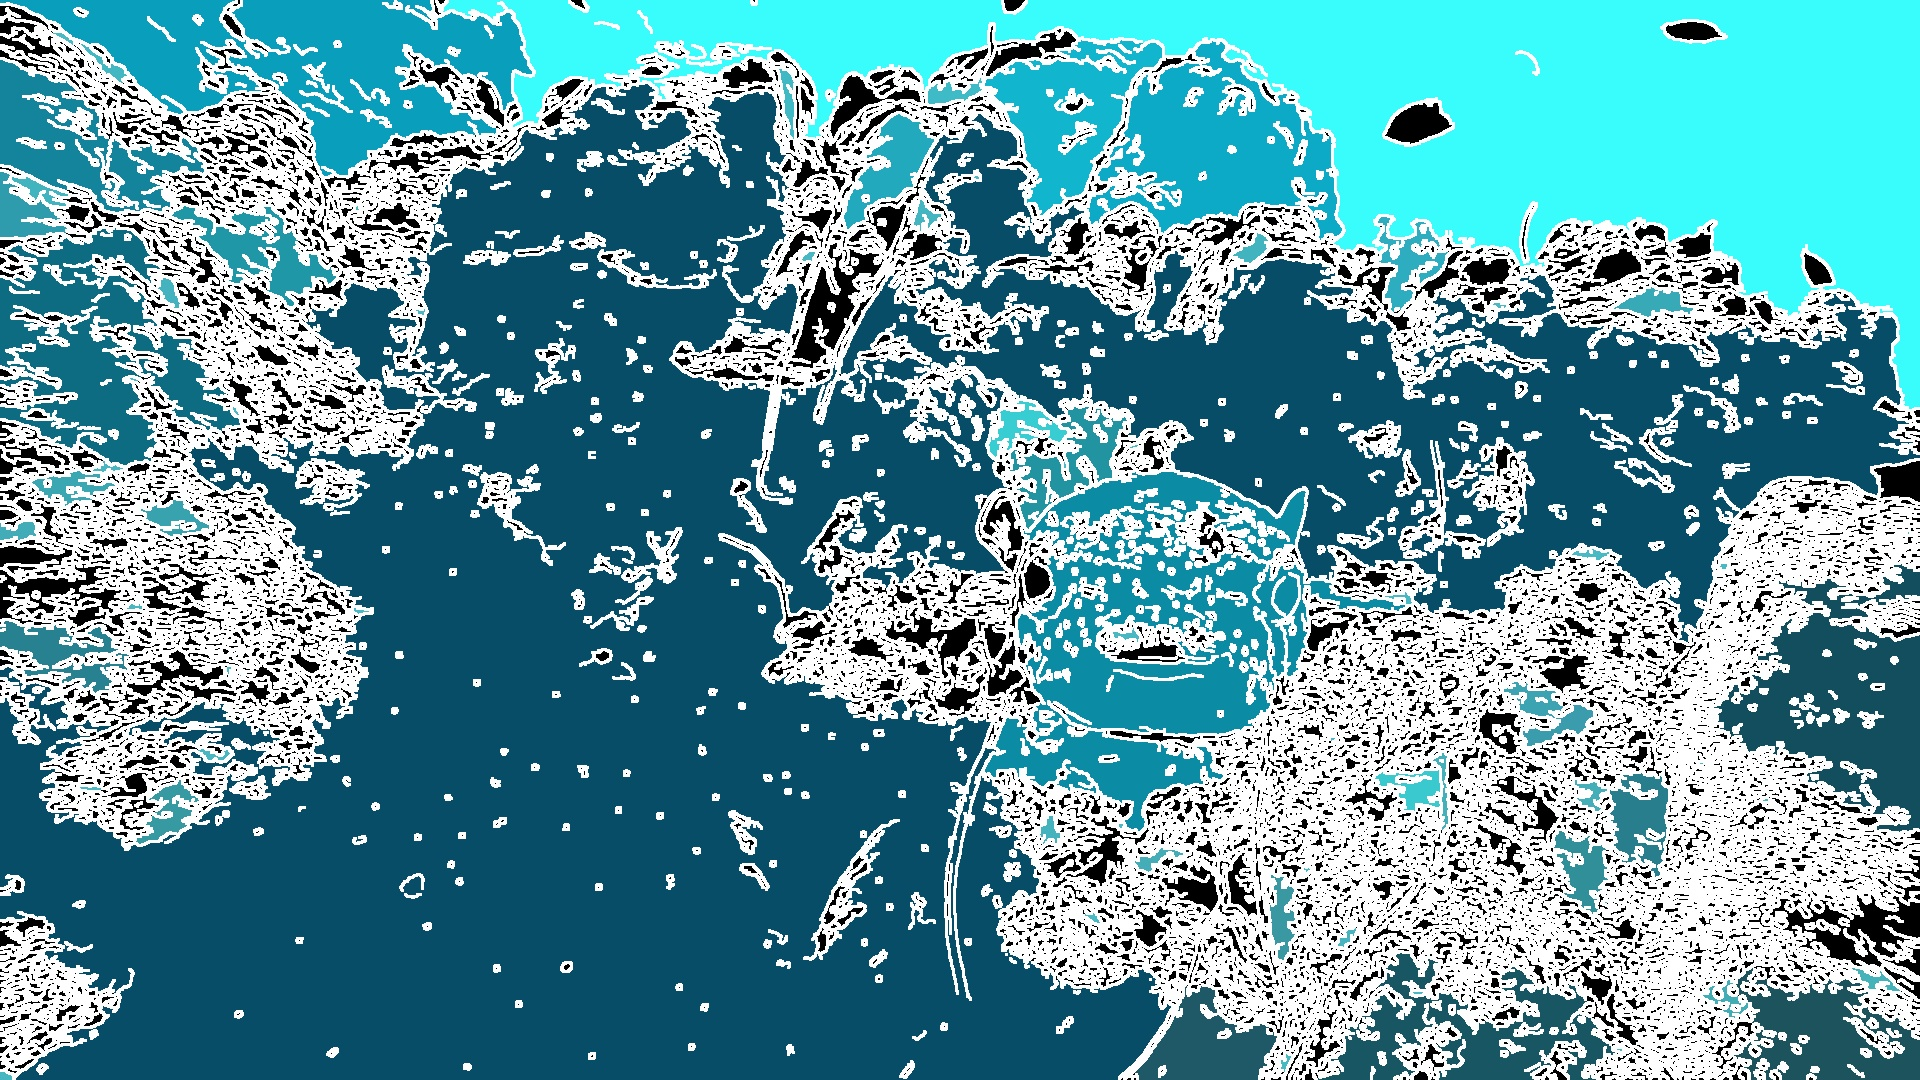
\includegraphics[width=0.45\textwidth]{Figures/pufferfishDA.jpg} \\
        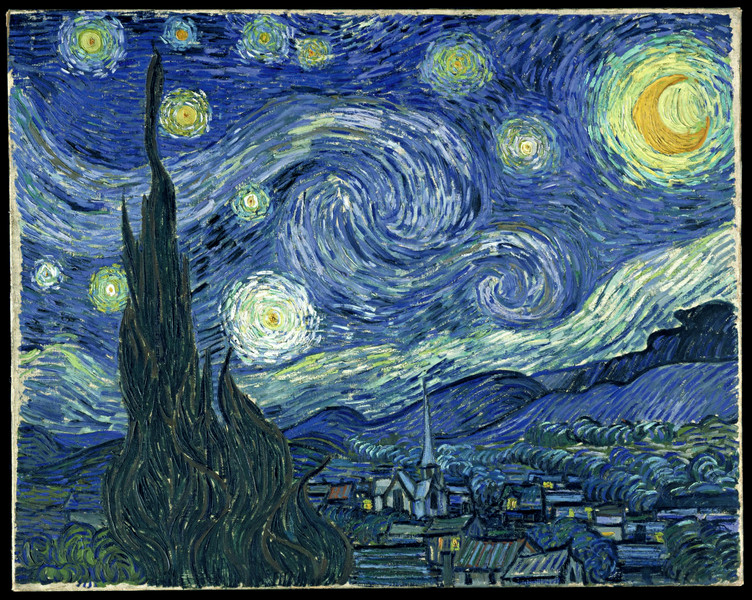
\includegraphics[width=0.45\textwidth]{Figures/starry_night.jpg} &
        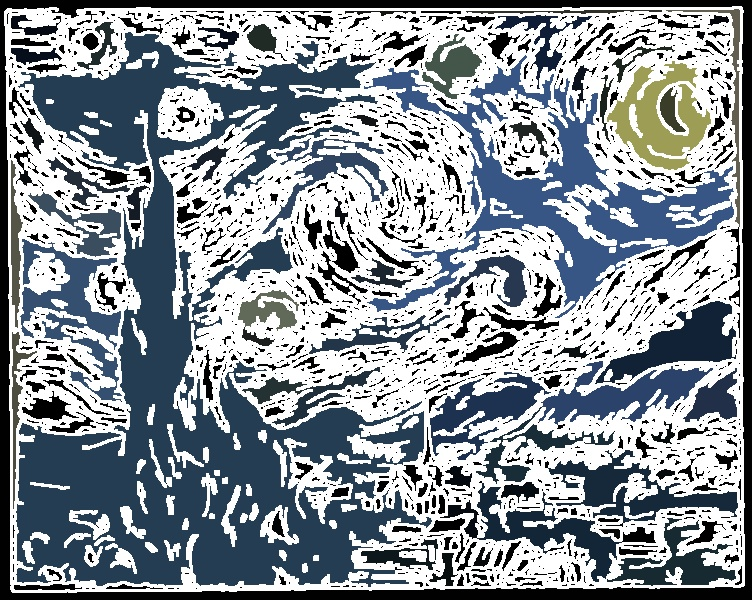
\includegraphics[width=0.45\textwidth]{Figures/starry_nightDA.jpg} 
    \end{tabular}
    \caption[Additional examples of the full abstraction process]{Additional examples of the full abstraction process. The top image (provided by OpenCV) is very simple, so the abstraction gives clean and easily recognisable results. The middle image (provided by fellow student Tom Darlison) was selected due to its limited colour palette and poor focus to test the limits of the process. While the image has mostly filled to a single colour, the pufferfish, rocks, coral, background fish, and open water are all identifiable. The bottom image (provided by OpenCV) was selected due to the extreme number of edges, due to the very clear brush strokes. Once the Canny threshold was turned down considerably, the result was recognisable as Starry Night, though much of the image has been overwhelmed by the edge detection lines. It can be concluded from these tests that the data abstraction process is effective at producing recognisable images, however the difficulty in interpreting the abstracted images is heavily dependant on the focus and complexity of the image.}
    \label{fig:FinalExtras}
    \end{center}
\end{figure} % Appendix Title
	
\chapter{Contour Based Seed Point Location}
\lhead{\emph{Contour Based Seed Point Location}}
\label{appendix:contour}

The ideal place to aim to flood fill a space from would be the centre point of the space. OpenCV provides the functionality to take the Canny output image (a matrix of colour values) and convert it into a set of contours. Contours are line objects stored in a hierarchical structure and have functions that can provide the centre point of each contour. Although the centre points of the contours will not map exactly to the centre points of the space, they are close enough approximations to flood fill from (Figure \ref{fig:ContourCentres}).

Unfortunately, due to a combination of the processing time required to convert the lines into contours and the number of contours produced that have no impact on the spaces left to be flood filled, this method is too resource heavy to produce 10 fps on a laptop, therefore is also too resource heavy for use on the raspberry pi.

\begin{figure}[H]
    \begin{center}
    \begin{tabular}{ c c }
        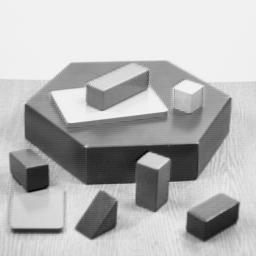
\includegraphics[width=0.31\textwidth]{Figures/blox.jpg} &
        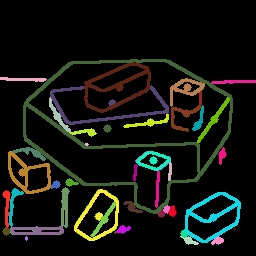
\includegraphics[width=0.31\textwidth]{Figures/ContourCentres.jpg}
    \end{tabular}
    \caption[Demonstration of contour centre point location]{Demonstration of contour centre point location. The original image (provided by OpenCV) on the left has been Canny edge detected, these edges have converted into contours, and the centre points of these contours located. The results of this are displayed on the right, with each contour and its corresponding centre point in a different colour. It can be observed that the centre points provide adequate coverage of the black spaces in the image to be used as seed points for flood filling.}
    \label{fig:ContourCentres}
    \end{center}
\end{figure}
 % Appendix Title

\chapter{Algorithm Performance Test Images}
\lhead{\emph{Algorithm Performance Test Images}}
\label{Appendix:scenes}
        
\begin{figure}[ht]
    \begin{center}
    \begin{tabular}{ c }
        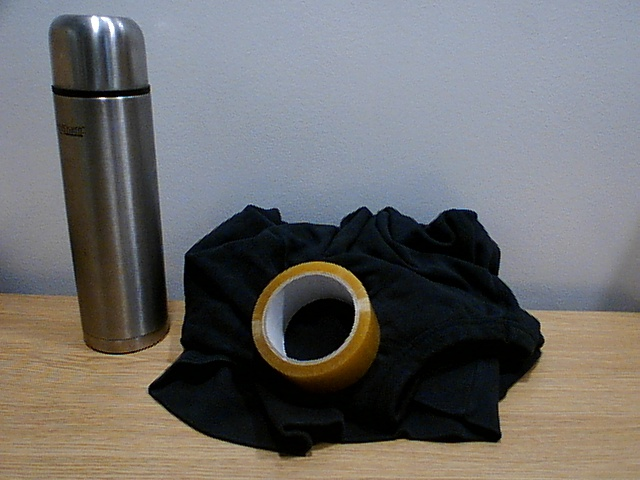
\includegraphics[width=0.6\textwidth]{Figures/simple.jpg} \\
        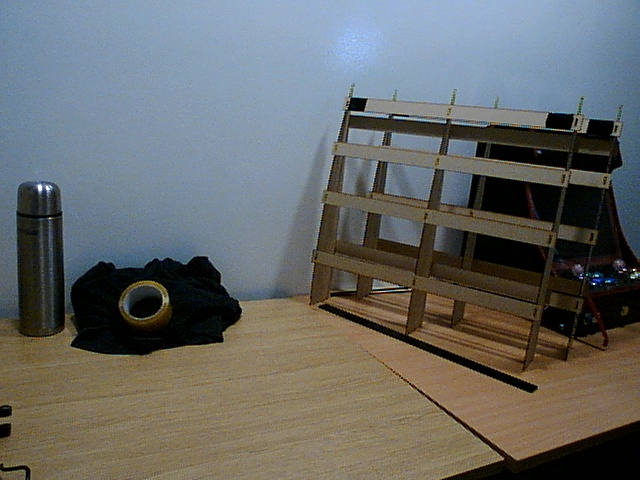
\includegraphics[width=0.6\textwidth]{Figures/medium.jpg} \\
        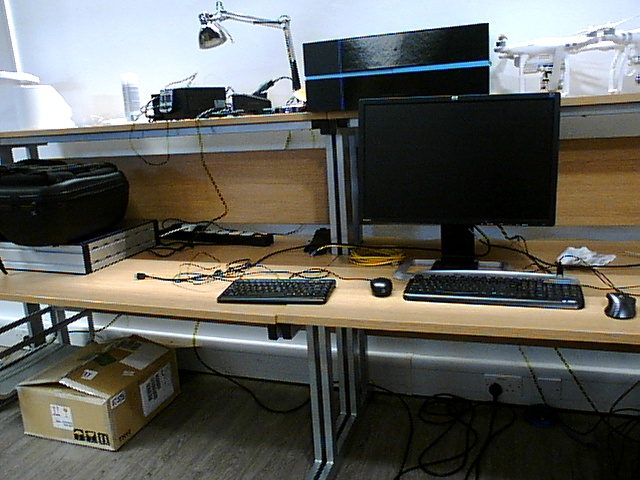
\includegraphics[width=0.6\textwidth]{Figures/complex.jpg} 
    \end{tabular}
    \caption[Images of Algorithm Performance Test Scenes]{Images of Algorithm Performance Test Scenes. From top to bottom, these are images of the simple scene, medium scene, and complex scene.}
    \label{fig:scenes}
    \end{center}
\end{figure} % Appendix Title

\chapter{Rover Hardware Breakdown}
\lhead{\emph{Rover Hardware Breakdown}}
\label{appendix:hardware}



\chapter{Vectorization}
\lhead{\emph{Vectorization}}
\label{appendix:vectorization}

As edge detected images consist of white lines on a black background, it would be logical to consider vector graphics as a storage method for wireless transmission. Vector graphics is the storage of images as line drawing and space filling instructions, allowing scaling to any size. When testing this, Potrace \cite{potrace} was used to convert the edge detected image bitmaps into encapsulated postscript documents (Figure \ref{fig:potrace}). 

\begin{figure}[H]
    \begin{center}
    \begin{tabular}{ c c }
        \multicolumn{2}{c}{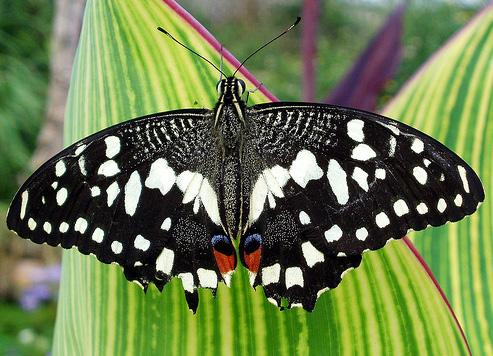
\includegraphics[width=0.4\textwidth]{Figures/butterfly.jpg}} \\
        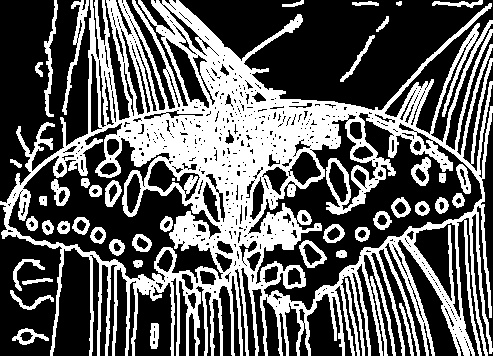
\includegraphics[width=0.4\textwidth]{Figures/butteredge.jpg} &
        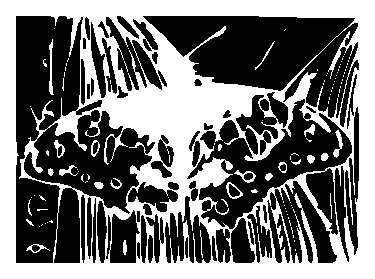
\includegraphics[width=0.4\textwidth]{Figures/butter.eps}
    \end{tabular}
    \caption[Conversion to Vector Graphics]{Conversion to Vector Graphics. While the vectorised image (bottom right) is clearly of the edge detection (bottom left), it utilises heavy approximation.}
    \label{fig:potrace}
    \end{center}
\end{figure}

When the documents were received by the server, they were converted back to OpenCV bitmaps using a custom interpreter built for the project. Both due to the approximation applied by Potrace and the custom interpreter not including all the necessary functions to accurately convert the vector files back to bitmaps, the final result loses much of its accuracy to the original image (Figure \ref{fig:potracecomp}). Due to the high edge accuracy requirements of producing a depth map from edge detected images, this method was discarded in favour of standard image compression. 

\begin{figure}[H]
    \begin{center}
    \begin{tabular}{ c c }
        
\includegraphics[width=0.4\textwidth]{Figures/buttercan.jpg} &
        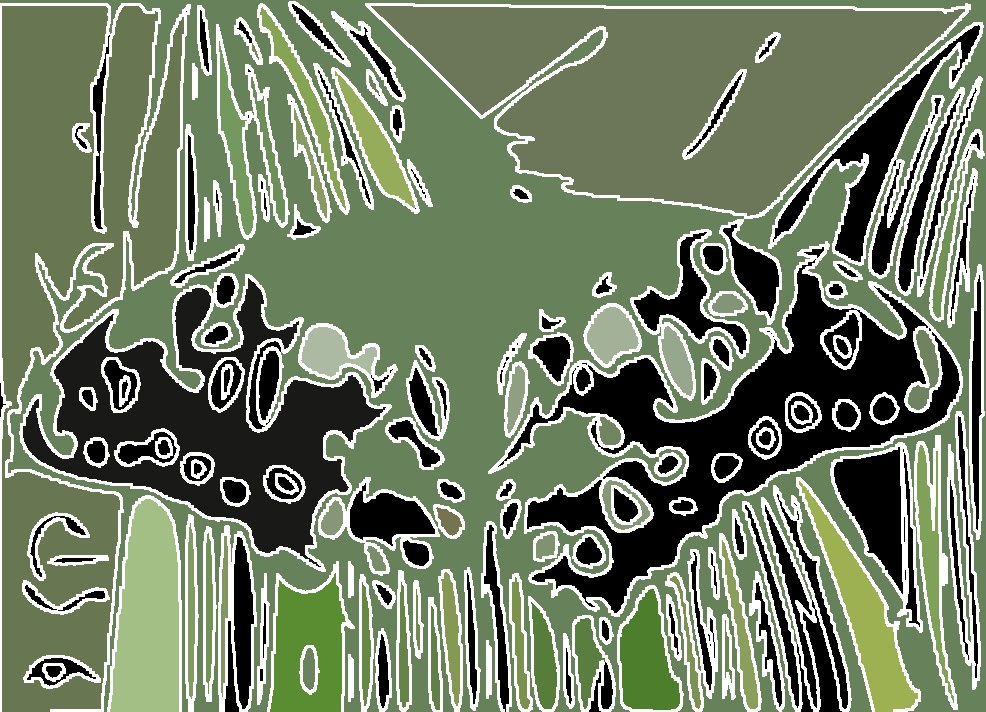
\includegraphics[width=0.4\textwidth]{Figures/butterred.jpg}
    \end{tabular}
    \caption[Comparison of Vector and Bitmap Accuracy]{Comparison of Vector and Bitmap Accuracy. Once the vector image has been converted back into a bitmap (right), it has lost much of its resemblance to the original image. A comparison to the image that results from transmitting compressed bitmaps (left) shows the sheer number of edges that have been either lost or combined together.}
    \label{fig:potracecomp}
    \end{center}
\end{figure}

\chapter{Project Brief}
\lhead{\emph{Project Brief}}
\label{appendix:brief}

\begin{center}
\textbf{Using Data Abstraction and Inter-Frame Interpolation for Low Data Rate Communication Between a 3D Camera and VR Headset} \\
Adam Melvin am20g15@soton.ac.uk \\
Klaus-Peter Zauner kpz@soton.ac.uk
\end{center}

There are many challenges, such as monitoring hostile environments, that call for the use of remotely controlled robots. Often in these scenarios, it would be useful to be able to view the environment with a sense of depth to better understand the scale, and dangers, of the robot’s surroundings. This can be provided through the use of a 3D camera on the robot and Virtual Reality (VR) goggles, however due to the minimum frame rate that can be displayed in a VR headset without causing motion sickness in the user being 60fps (optimally 90fps is preferable), a comfortable and useful experience would often require an unfeasibly high wireless data rate.

The aim of this project is to significantly reduce the data rate required to be transmitted between a robot and teleoperator through the use of data abstraction and inter-frame interpolation. A 3D camera rig mounted on a remotely controlled rover is to take around 10 pictures per second, then they are reduced down to the minimum amount of data required to identify the objects in the environment. These much smaller images are sent wirelessly to a server, where they are used to create a 3D map of the environment. These 3D maps are analysed and intermediate frames are estimated to increase the frame rate from 10fps to 60-90fps. This much higher frame rate estimated map of the environment can then be displayed in the VR headset through the use of a video game engine. Although the estimated frames will not accurately represent the real world, the comfort they provide the user will allow them to focus on the transmitted information without feeling ill.

A simple rover and off-the-shelf VR equipment will be used as a foundation for the system. Different camera systems and interpolation algorithms will be tested on this foundation to discern the setup that produces the best ratio between data rate and usability.


\chapter{Gantt Charts}
\lhead{\emph{Gantt Charts}}
\begin{landscape}
\begin{figure}[ht]
    \begin{center}
    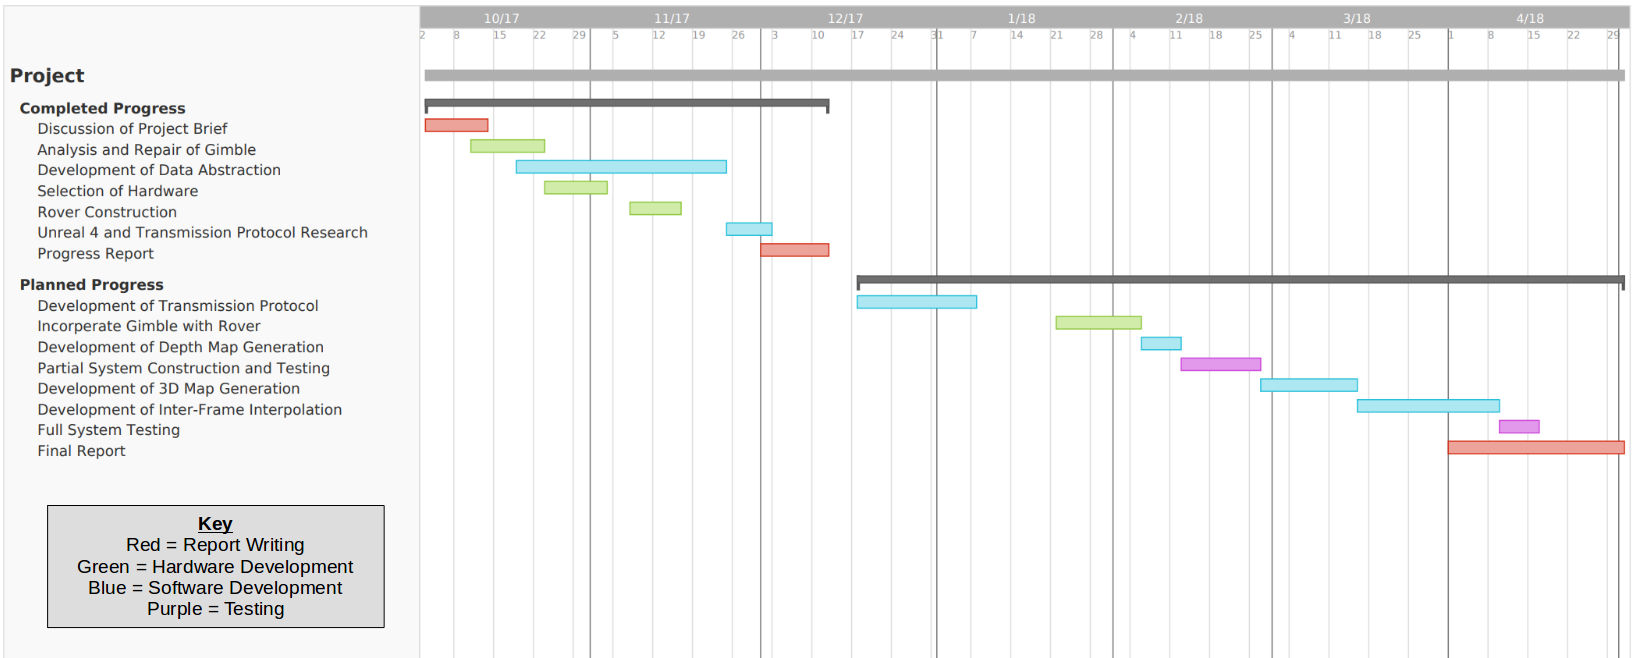
\includegraphics[width=1.5\textwidth]{Figures/ganttfinal.png}
    \label{fig:GanttChart}
    \end{center}
\end{figure}
\end{landscape} % Appendix Title

\chapter{Risk Assessment}
\lhead{\emph{Risk Assessment}}
\label{appendix:risk}

\begin{landscape}
\begin{figure}[ht]
    \begin{center}
      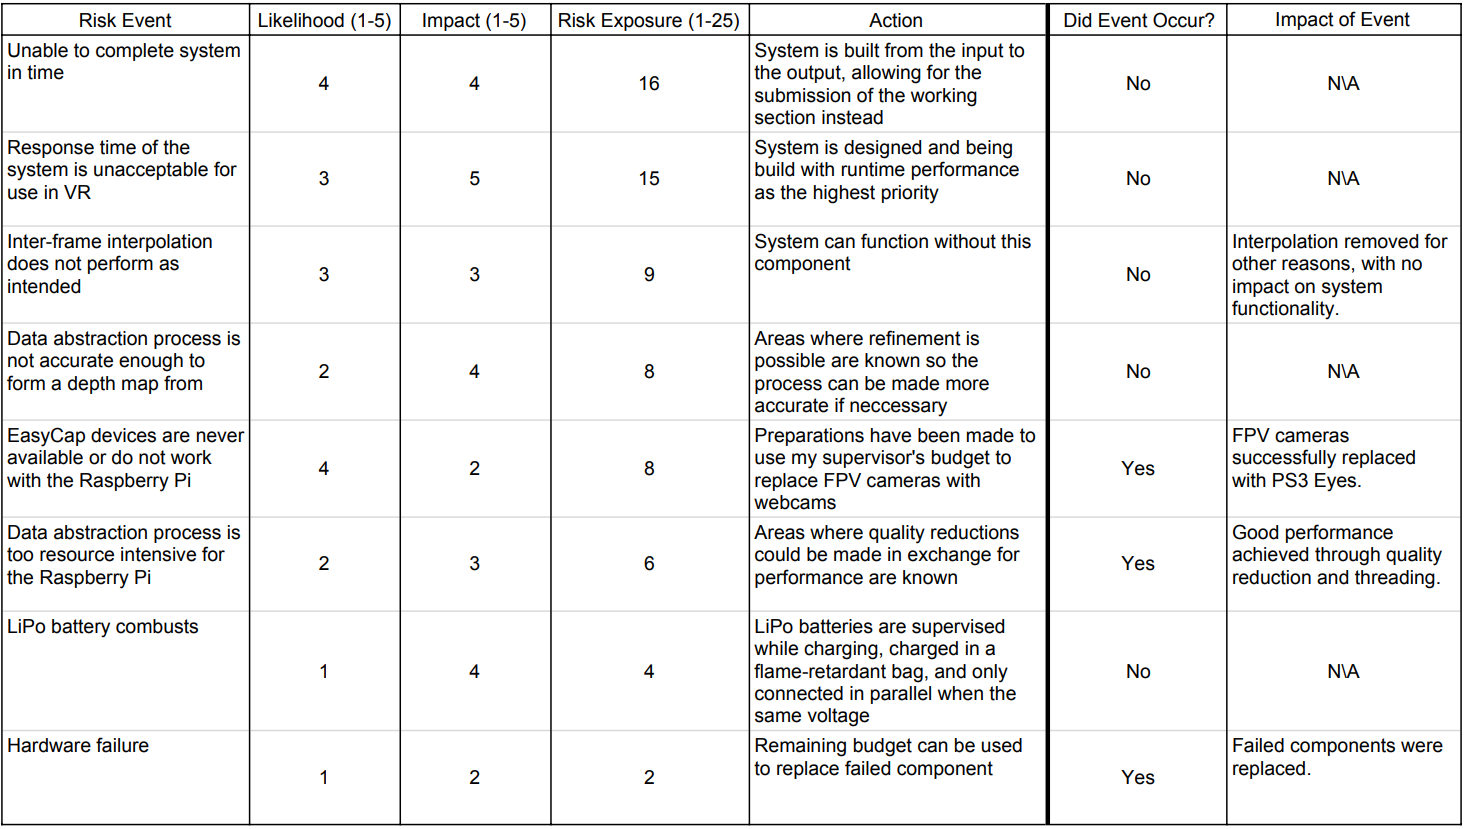
\includegraphics[width=1.5\textwidth]{Figures/risk.png}
      \caption[Risk Assessment]{Risk Assessment. Left of the thicker line is the original risk assessment from the interim report, and right of the thicker line is the end of project evaluation of the risk assessment.}
      \label{fig:Risk}
    \end{center}
\end{figure}
\end{landscape} % Appendix Title

\chapter{Design Archive Contents}
\lhead{\emph{Design Archive Contents}}
\label{appendix:archive}

 % Appendix Title



\end{document}  % The End
%% ----------------------------------------------------------------